\chapter{LITERATURE REVIEW}\label{litreview}

\begin{abstract}
Conducting inference is a cornerstone upon which the practice of statistics is based. As such, a large portion of most introductory statistics courses is focused on teaching the fundamentals of statistical inference. The goal of this study is to make a formal comparison of learning outcomes under the traditional and simulation-based inference curricula. A randomized experiment was conducted to administer the two curricula to students in an introductory statistics course.  The results indicate that students receiving the simulation-based curriculum have significantly higher learning outcomes for confidence interval related topics. While the results are not comprehensive in assessing the effect on all facets of learning, they indicate that learning outcomes for core concepts of statistical inference can be significantly improved with the simulation-based approach. 

\end{abstract}



%---------------------------------------------------------------------------
\section{Introduction}
\label{intro}

Conducting inference is a cornerstone upon which the practice of statistics is based. As such, a large portion of most introductory statistics courses is focused on teaching the fundamentals of statistical inference. In recent years the approach by which to teach inference in introductory statistics courses has been the topic of growing discussion.  The traditional approach to inference curriculum is focused on distributional theory-based methodology, often characterized by use of distributional assumptions, formulas and tables. A modern alternative is a simulation-based approach to the inference curriculum. The simulation-based approach utilizes tactile and computational simulation to run inferential techniques such as bootstrapping for confidence intervals and simulation-based hypothesis testing. Many proponents of the simulation-based inference curriculum argue that this allows students to be exposed to the core concepts of the inference without first requiring the understanding of theoretical probability distributions. 

The focus of the following study is to make a formal comparison of learning outcomes under the traditional and simulation-based inference curricula.  The learning outcomes for concepts surrounding inference with confidence intervals and hypothesis testing are of primary interest.  A randomized experiment was conducted to administer the two curricula to students in an introductory statistics course. The experimental design allows for causal inference to be drawn about the effect of curriculum type on the learning outcomes. The results indicate that significant improvement in learning outcomes for confidence interval related topics are achieved using the simulation-based teaching methods.
%---------------------------------------------------------------------------
\section{Literature Review}
\label{litreview}

With the goal to make proper comparison of traditional versus simulation-based curricula for introductory statistical courses, we must first view where each approach stands within the constant evolution of statistics education. Using the term ``traditional'' to describe the current standard for introductory statistics course curriculum is relative to only the last two decades. Moore chronicled the reform movement of statistic education of the 1980's and 1990's as a period of drastic change in the introductory statistics classroom.  The curriculum expanded greatly from a course dominated by theory-based inference methodology to the inclusion of the topics of data exploration, data production, model diagnostics and simulation.  The content change indicated a shifting emphasis toward conceptual understanding and applied statistics.  Moore also stated, ``(w)hat is striking about the current reform movement is not only its momentum but the fact that it centers on pedagogy as much as content'' \citep{Moore1997}. The pedagogical push toward active learning was combined with content change and the increasing use of technology to form what may be referred to now as the traditional introductory statistics curriculum. 

The tenets of the statistics education reform movement were formalized in the Guidelines for Assessment and Instruction in Statistics Education (GAISE) reports for pre-K-12 \citep{GAISEk12} and introductory college courses \citep{GAISEcollege}. Six recommendations were made in the executive summary of the GAISE college report: emphasize statistical literacy and thinking, use real data, stress conceptual over procedural understanding, foster active learning, use technology for both learning and analysis, and use assessment as part of the learning process.  In the past decade these principles have been widely adopted in statistics education with a noteworthy increase in technological integration.  Technology in the statistics classroom now regularly takes the form of applets, graphing calculators, multimedia materials, and educational, analytical and graphical software (\citealt{Chance2007}; \citealt{Rubin2007}).  Technological proliferation in the statistics classroom came as a result of technologically receptive statistics educators taking advantage of computation that has become cheaper and more accessible.  A large survey of introductory statistics instructors found that 76\% of the instructors usually or always require students to use a computer program to explore and analyze data, and 90\% of the instructors report a high level of comfort using computer applications to teach introductory statistics \citep{Hassad2013}.  

Amidst the drastic increase in the use of technology in introductory statistics education there has been a growing group of educators who believe that the curriculum reform has stopped short of the possibilities that computation can provide.  Cobb argues that statistics education has done well to adopt technology to displace tedious calculation but has not effectively changed the approach to teaching inference.  Cobb strongly articulates a call for statistics instructors to use simulation-based methods for teaching inference to replace the traditional approach to inference using theory-based methodology.  He states, ``(o)ur curriculum is needlessly complicated because we put the normal distribution... at the center of our curriculum, instead of the core logic of inference at the center'' \citep{Cobb2007}.  If we view the introductory statistics course as a constrained optimization problem with statistical literacy and conceptual understanding of inference as the items to maximize, then removing the burden of learning the normal distribution will present the opportunity for more time spent learning core concepts \citep{Carver2011}.   In recent years, curricula for using a simulation-based approach to inference have been developed by a number of groups of statistics educators (\citealt{ISI}; \citealt{Lock5}; \citealt{CATALST};  \citealt{Carver2011}).  

There has been research done on the efficacy of simulation-based inference curricula; however, due to the recency of the curricula development most of this preliminary research has been observational.  Budgett, Pfannkuch, Regan \& Wild conduct a case study on a small group of students receiving a simulation-based curriculum and found significant learning gains using pre and post testing based on the Comprehensive Assessment of Outcomes in a First Statistics Course (CAOS).  This study does not however attempt to make a comparison between the simulation-based approach and traditional approach to teaching inference \citep{Budgett2013}. Another pair of studies make comparisons on both learning outcomes and learning retention between the two types of curricula. Tintle, VanderStoep, Holmes, Quisenberry and Swanson found weak evidence for an overall improvement in learning outcomes and significant improvements within the topic of hypothesis testing for the cohort of students receiving the simulation-based curriculum, but the lack of random assignment of student to cohort obstructs the ability to draw any causal conclusions \citep{Tintle2011}.  Tintle, Topliff, VanderStoep, Holmes and Swanson then found significant evidence for improvements to learning outcome retention after four months for students receiving the simulation-based inference curriculum, but again self-selection of students to cohort prevents establishing a causal link \citep{Tintle2012}.  

The preliminary research shows promising results for the simulation-based approach to teaching statistical inference.  A more rigorous experimental approach to comparing the traditional and simulation-based curricula has been taken in this study in order to establish a causal effect of curriculum on learning outcomes. Section 3 explains the structure and methodology implemented in the educational experiment and the measurement of student learning.  Section 4 details the model based approach for assessing the effect of curriculum on specific learning outcomes.  Lastly, we discuss the study findings and explore the implications for designing future introductory statistics curricula.
%---------------------------------------------------------------------------
\section{Methodology}
\label{methods}

The subjects for this study were students enrolled in two sections of the Introduction to Statistics, Stat 104, course at Iowa State University in the spring semester of 2014. Stat 104 is an introductory statistics course tailored for students in the agricultural and biological sciences. Of the 112 students to complete the course, 101 students consented to the release of their course data for the purposes of this study.   The students who did not consent were treated identically to those who consented, but their data was omitted from the analysis that follows.  Students from both sections were randomly assigned to one of the two inference curriculum treatments, creating cohorts A,C and B,D, respectively. Cohorts A and B were exposed to the simulation-based curriculum; while the cohorts C and D were exposed to the traditional curriculum. Student cohorts were the basic units to which room assignments, instruction and curriculum treatments were applied.

The course was administered by the authors in a co-teaching setting for students from all cohorts. The course schedule involved two hours of lecture and two hours of lab per week.  The co-teaching strategy was employed as an intentional attribute of the experimental design. The following subsections will detail the curriculum outline for each cohort of students, the experimental design for administering the curricula using the strengths of the co-teaching setup and the data collected for analysis.
%-----------------------------------------------------
\subsection{Curricula Structures}
\label{curric}

To compare the learning outcomes for students receiving the traditional and simulation-based inference curricula we first needed to prepare a curriculum for each approach.  Both curricula needed to satisfy the course guidelines set by the Department of Statistics at Iowa State University, covering the following topics: univariate and bivariate descriptive statistics, linear regression, experimental design, basic probability rules, the binomial distribution, the normal distribution, sampling distributions, and inference on means and proportions. Each curriculum was composed of lecture, corresponding lecture notes, weekly lab assignments designed for groups of four to five students, weekly homework assignments, a midterm exam and a cumulative final exam.  The curricula materials for the course did not require the use of a textbook, however specific textbooks that roughly follow the structure of each curriculum were recommended as supplementary study materials (\citealt{AgrestiFranklin}; \citealt{Lock5}).

Figure~\ref{fig:CurricSched} outlines how these topics were structured within a weekly schedule for the sixteen week semester for each curriculum.  Note that students from all cohorts were exposed to an identical curriculum for all non-inference related topics in the course. This includes identical lecture, course notes, homework assignments, lab assignments and midterm exam during the first half of the semester.

Starting at week 9 the curricula diverge into their respective approaches to inference.  Cohorts A and B began the simulation-based inference curriculum in week 9 by first learning the concepts of sampling distributions then used computer simulation and sampling variability as a basis for exploring inference using bootstrap confidence intervals and simulation-based tests.  To be specific, confidence intervals were constructed by estimating the standard error using the standard deviation of the bootstrap distribution, not through percentile-based bootstrap methods.  Lectures, homework and labs for these cohorts utilized the StatKey software package \citep{Lock5} to conduct the simulation-based inference. The simulation-based curriculum then covered normal distributions and how they could be used to conduct inference on means and proportion.  While many advocates for simulation-based methods may argue that the normal distribution should be pushed to a second course in statistics, course guidelines required that all students of this introductory statistics course be taught theory-based inference methodology.  

\begin{figure}[hbtp]
\centering
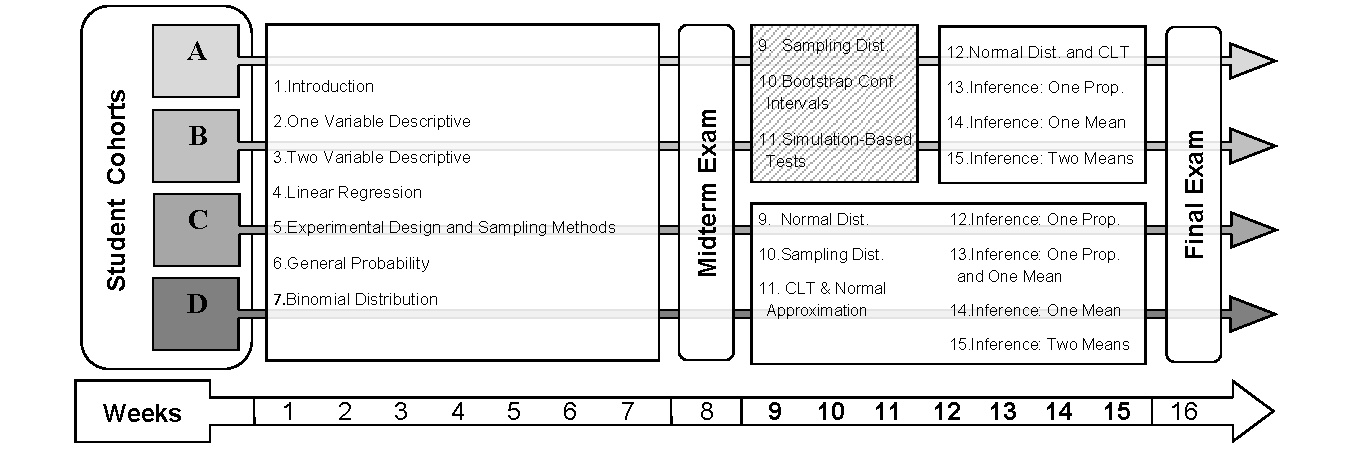
\includegraphics[keepaspectratio=true, width=1\textwidth]{figure/CurriculaPaths2.pdf}
\caption{\label{fig:CurricSched} Curricula Schedules}
\end{figure}

% Cohorts C and D progressed through the traditional approach by first learning the normal distribution and use of the normal tables. They were then introduced to applications of the normal approximation within inference.  The traditional curriculum utilized simulation to display concepts, but only to the extent of demonstrating that sampling distributions can be approximated by normal distributions under certain conditions.  
% 
% During the second half of the semester the lectures, course note, homework and lab assignments differed between the two curricula.  However, homework and lab assignments were kept similar when they covered similar topics.  For example, all cohorts covered the topic of sampling distributions so the lab assignments were nearly identical between the two groups with the exception of a question pertaining to the normal approximation included for the traditional cohorts.  By the end of the semester all cohorts covered how to conduct inference using normal theory; however cohorts A and B additionally learned the core concepts of inference using simulation-based methods prior to learning traditional theory-based inference methods.  
% 
% %-----------------------------------------------------
% \subsection{Experimental Design}
% \label{design}
% 
% The logistics of administering a course with two distinct curricula and four cohorts of students required a well-structured design and creative scheduling on several fronts.  The primary objectives for the experimental design were to eliminate differences in non-inference related curriculum administration to the extent possible, remove the confounding instructor effect on each curriculum and to mitigate the effect of unknown lurking variables through random assignment of students to curricula.  
% 
% Students were randomly assigned to cohorts during the first week of the course.  Of the 101 students who completed the course and consented to the release of their data there were 50 students in the traditional treatment group and 51 students in the simulation-based treatment group. It is also worthwhile to note that of the 4 students to drop the course, all did so prior to week 9; thus, we can safely assume that the inference curriculum treatment did not play a role in the drop. All students who began the inference curricula completed the course.
% 
% Students were exposed to identical lecture and lab instruction for the first half of the semester and then diverge into two separate lecture and lab settings for the second half of the semester. This was done to make the experience as similar as possible such that both treatment groups would have the same exposure to terminology and ideas leading up to the inference topics. We could not reassign students to lecture and lab times different than the times for which they enrolled, which meant the logistics of the design required preemptive room scheduling and course time scheduling preparations.  By working with the department chair and course coordinator before students enrolled into sections, we were able to schedule two sections of the course to have identical lecture times but separate lab times. Special room scheduling was required because all students needed to attend the same lecture and lab rooms for the first half of the semester then split into separate lecture and lab rooms after the midterm.  This room and course time scheduling allowed for students to be divided into cohorts and attend the lecture or lab specific to their curriculum.  The lecture and lab room schedules for each cohort are displayed in Figure~\ref{fig:InstSched}.
% 
% \begin{figure}[hbtp]
% \centering
% 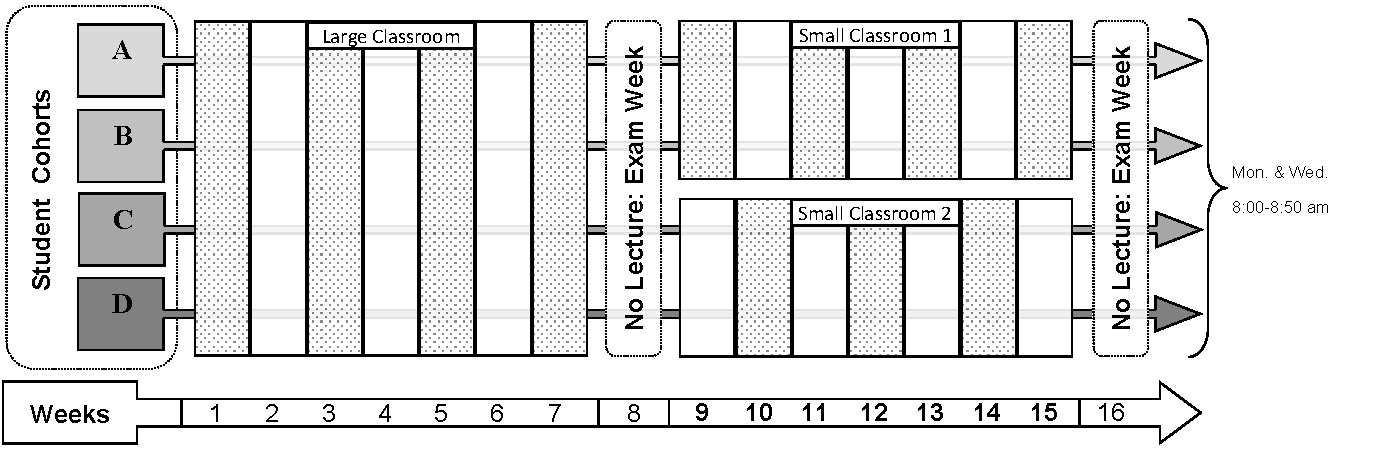
\includegraphics[keepaspectratio=true, width=1\textwidth]{figure/LectureInstructionWithRooms.pdf}\\
% \vspace{.5cm}
% 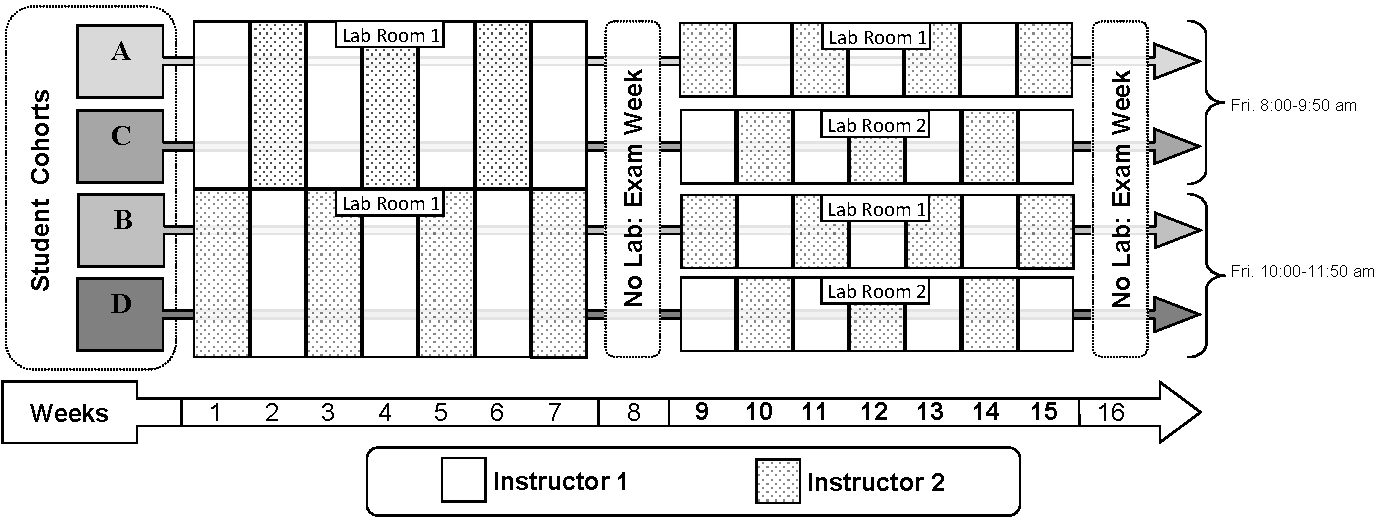
\includegraphics[keepaspectratio=true, width=1\textwidth]{figure/LabInstructionWithRooms.pdf}
% \caption{\label{fig:InstSched} Instructor and Room Schedule}
% \end{figure}
% 
% 
% Assigning one instructor to each curriculum would confound the instructor effect and the curriculum effect.  To avoid confounding, each treatment group would need to receive instruction from both instructors.  An alternating weekly schedule was decided upon to spread out the instructor effects over both curricula. A coin was flipped to decide how to match the instructor to the curriculum when the alternation was initialized. The lecture and lab instruction schedules for each cohort can also be found below in Figure~\ref{fig:InstSched}. Note that each figure has student cohort and times fixed across all weeks, reflecting the unchanged time structure that each student enrolled into. The instructors and room locations are what changed throughout the course. 
% 
% %-----------------------------------------------------
% \subsection{Data Collection}
% \label{datacollect}
% 
% In order to measure learning outcomes for specific inference concepts we utilized question sets from the Assessment Resource Tools for Improving Statistical Thinking (ARTIST) for the topics of confidence intervals and hypothesis testing \citep{ARTIST}.  The ARTIST scaled question sets each consist of 10 multiple choice questions that are geared toward critical thinking about the inference topic.  These questions were administered as part of the written final exam for all students on the same day and time. The ARTIST scaled scores for the topics of confidence interval and hypothesis testing were recorded for each student. The multiple choice questions for the ARTIST scaled topics can be found in Appendix~\ref{appendA}.
% 
% The final exam also included two problems that tested the student's ability to conduct statistical inference in an applied setting using theory-based methodology. Each problem was based on a hypothetical scenario where data has been collected and inference needed to be conducted using the traditional approach using formulas and tables. The first problem provided data summaries and students needed to construct and interpret a confidence interval for a single population mean. The second problem required students to conduct a hypothesis test for a single proportion based on another set of data summaries. The applied inference problem scores for each student are not used for the primary analysis on learning outcomes but are included for an interesting peripheral analysis on student ability to conduct inference using traditional theory-based methods. The applied inference problems and grading rubrics can also be found in Appendix~\ref{appendA}. The exams were graded blindly, with no identifying information of the student or treatment visible during the grading process.
% 
% In addition to the ARTIST and applied inference question scores, data were collected from the first eight weeks of the course -- prior to student exposure to an inference curriculum. We have scores from homework assignments 1 to 7, lab assignments 1 to 7 and the midterm exam for each student. The midterm exam questions and grading rubrics can be found in Appendix~\ref{appMidtermExamQuestions}. Since all of these items were administered and graded equivalently for all students before being assigned to a curricula, the scores from these weeks will be referred to as the ``pre-treatment measurements''. Lastly, the data include the cohort to which each student belonged.
% 
% The research proposal approved by the Institutional Review Board specified that students' data would be entirely deidentified following the course, including all demographic information.  At the conclusion of the semester the data for the 101 students who consented to the release of their data were saved, with names and identity information removed, to a spreadsheet.  The deidentified student data was imported to \texttt{R} for the analysis described in Section~\ref{analysis} below. 
% 
% 
% %-----------------------------------------------------
% \subsection{Data Summary}
% \label{dataSummary}
% 
% The ARTIST and applied inference question scores from the final exam are the response variables on which we wish to compare the groups of students from the two inference curricula. Figure~\ref{fig:ScoreHistsByGroup} displays the histogram, mean and standard deviation for each response variable, separated by curricula.  Midterm exam scores as also included in order to provide a comparison of the curricula groups using a pre-treatment measurement. 
% 
% <<ScoreHistsByGroup, echo=FALSE , warning=FALSE, fig.width=15, fig.height=8, out.width='1\\linewidth', fig.pos='h',fig.align='center',fig.cap="Histograms and summary statistics of scores separated by curricula group.">>=
% dat$treatment <- "Simulation-Based"
% dat$treatment[which(dat$room=="sweeney")] <- "Traditional"
% 
% smalldat <- dat[,c("treatment","midterm","ConfMC","HypMC","AppliedCI","AppliedHT")]
% meltsmall <- melt(smalldat, id=c("treatment"))
% trtsumstats <- ddply(dat, .(treatment), summarize,
%                    avgmidterm = round(mean(midterm),1 ), 
%                    sdmidterm = round(sd(midterm), 2 ), 
%                    avgConfMC = round(mean(ConfMC),1 ), 
%                    sdConfMC = round(sd(ConfMC), 2 ), 
%                    avgHypMC = sprintf("%.1f",round(mean(HypMC),1 )), 
%                    sdHypMC = round(sd(HypMC), 2 ), 
%                    avgAppliedCI = round(mean(AppliedCI),1 ), 
%                    sdAppliedCI = round(sd(AppliedCI), 2 ), 
%                    avgAppliedHT = round(mean(AppliedHT), 1 ), 
%                    sdAppliedHT = round(sd(AppliedHT), 2 )  ) 
% 
% titlesize =1.5
% xaxissize =1.3
% sumstatfont = 6
% yscale <- c(0,25)
% 
% 
% themeForMultHist <- theme(plot.margin=unit(c(1,0,1,0), "cm"),
%                           axis.title.y= element_blank() ,
%                           strip.text.y = element_text(size = rel(xaxissize)),
%                           #strip.background = element_blank(),
%                           plot.title = element_text(size = rel(titlesize)),
%                           axis.title.x = element_text(size = rel(xaxissize)))
% 
% 
% p1 <- qplot(midterm, data=dat, facets = treatment ~ ., binwidth=8, origin=4) + theme_bw()  +  
%   xlab("Score (Out of 100)") + ggtitle("Midterm Exam") +
%   #ylim(yscale) +
%   geom_text(aes(x, y, label=lab), 
%     data=data.frame(x=-1,y=12, lab=c(paste("mean =",trtsumstats[1,2]),paste("mean =",trtsumstats[2,2])) ,
%     treatment=c("Simulation-Based","Traditional")), hjust=0, vjust=1, size= rel(sumstatfont)  )  + 
%   geom_text(aes(x, y, label=lab), 
%     data=data.frame(x=-1,y=.85*12, lab=c(paste("sd =",trtsumstats[1,3]), paste("sd =",trtsumstats[2,3])) ,
%     treatment=c("Simulation-Based","Traditional")), hjust=0, vjust=1, size= rel(sumstatfont)    )+
%   themeForMultHist + 
%   scale_x_continuous(limits=c(-1, 100),breaks=seq(from=0, to=100, by=25))
% 
% p2 <- qplot(ConfMC, data=dat, facets = treatment ~ ., binwidth=1) + theme_bw() + 
%   xlab("Score (Out of 10)") + ylab("")  + ggtitle("ARTIST CI") +
%   #ylim(yscale) +
%   geom_text(aes(x, y, label=lab), 
%     data=data.frame(x=-1,y=12, lab=c(paste("mean =",trtsumstats[1,4]),
%                                     paste("mean =",trtsumstats[2,4])) ,
%     treatment=c("Simulation-Based","Traditional")), hjust=0, vjust=1 , size= rel(sumstatfont)   )  + 
%   geom_text(aes(x, y, label=lab), 
%     data=data.frame(x=-1,y=.85*12, lab=c(paste("sd =",trtsumstats[1,5]),
%                                     paste("sd =",trtsumstats[2,5])) ,
%     treatment=c("Simulation-Based","Traditional")), hjust=0, vjust=1, size= rel(sumstatfont)    )+
%   themeForMultHist + 
%   scale_x_continuous(limits=c(-1, 11),breaks=seq(from=0, to=10, by=2))
% 
% 
% p3 <- qplot(HypMC, data=dat, facets = treatment ~ ., binwidth=1) + theme_bw() + 
%   #ylim(yscale) + 
%   xlab("Score (Out of 10)") + ylab("")  +  ggtitle("ARTIST HT") +
%   geom_text(aes(x, y, label=lab), 
%     data=data.frame(x=-1,y=13, lab=c(paste("mean =",trtsumstats[1,6]),
%                                     paste("mean =",trtsumstats[2,6])) ,
%     treatment=c("Simulation-Based","Traditional")), hjust=0, vjust=1 , size= rel(sumstatfont)   )  + 
%   geom_text(aes(x, y, label=lab), 
%     data=data.frame(x=-1,y=.85*13, lab=c(paste("sd =",trtsumstats[1,7]),
%                                     paste("sd =",trtsumstats[2,7])) ,
%     treatment=c("Simulation-Based","Traditional")), hjust=0, vjust=1 , size= rel(sumstatfont)   )+
%   themeForMultHist + 
%   scale_x_continuous(limits=c(-1, 11),breaks=seq(from=0, to=10, by=2))
% 
% p4 <- qplot(AppliedCI, data=dat, facets = treatment ~ ., binwidth=1) + theme_bw() + 
%   #ylim(yscale) + 
%   xlab("Score (Out of 12)") + ylab("")  +  ggtitle("Applied CI") +
%   geom_text(aes(x, y, label=lab), 
%     data=data.frame(x=-1,y=24, lab=c(paste("mean =",trtsumstats[1,8]),
%                                     paste("mean =",trtsumstats[2,8])) ,
%     treatment=c("Simulation-Based","Traditional")), hjust=0, vjust=1 , size= rel(sumstatfont)   )  + 
%   geom_text(aes(x, y, label=lab), 
%     data=data.frame(x=-1,y=.85*24, lab=c(paste("sd =",trtsumstats[1,9]),
%                                     paste("sd =",trtsumstats[2,9])) ,
%     treatment=c("Simulation-Based","Traditional")), hjust=0, vjust=1 , size= rel(sumstatfont)   )+
%   themeForMultHist+ 
%   scale_x_continuous(limits=c(-1, 13),breaks=seq(from=0, to=12, by=4))
% 
% p5 <- qplot(AppliedHT, data=dat, facets = treatment ~ ., binwidth=1) + theme_bw() + 
%   #ylim(yscale) + 
%   xlab("Score (Out of 11)") + ylab("")  +  ggtitle("Applied HT") +
%   geom_text(aes(x, y, label=lab), 
%     data=data.frame(x=-1,y=19, lab=c(paste("mean =",trtsumstats[1,10]),
%                                     paste("mean =",trtsumstats[2,10])) ,
%     treatment=c("Simulation-Based","Traditional")), hjust=0, vjust=1 , size= rel(sumstatfont)   )  + 
%   geom_text(aes(x, y, label=lab), 
%     data=data.frame(x=-1,y=.85*19, lab=c(paste("sd =",trtsumstats[1,11]),
%                                     paste("sd =",trtsumstats[2,11])) ,
%     treatment=c("Simulation-Based","Traditional")), hjust=0, vjust=1 , size= rel(sumstatfont)   )+
%   themeForMultHist + 
%   scale_x_continuous(limits=c(-1, 12),breaks=seq(from=0, to=12, by=4))
% 
% grid.arrange(textGrob("Count", rot = 90, gp = gpar(cex = 1.5)),
%              arrangeGrob(p1,p2,p3,p4,p5, nrow=1), 
%              #arrangeGrob(textGrob("Simulation-Based", vjust = 1,
%              #                     gp = gpar(cex = 1.5), rot = 90),
%              #            textGrob("Traditional", vjust = 1, 
%              #                     gp = gpar(cex = 1.5), rot = 90)),
%              widths=unit.c(unit(2, "lines"), unit(1, "npc") - unit(2, "lines")),
%              nrow=1
%              )
% @
% \vspace{.05in}
% In Figure~\ref{fig:ScoreHistsByGroup}, we see that the midterm exam scores are very similarly distributed for each group; with the traditional curriculum group scoring only slightly higher on average than the simulation-based curriculum group. This similarity is expected -- and desirable -- because the midterm was conducted prior to the treatment being administered, and the class materials and instruction were designed to be identical at that stage of the course.
% 
% Comparing the distributions in Figure~\ref{fig:ScoreHistsByGroup} we see that the simulation-based inference group had a higher average score than the traditional inference group on both of the ARTIST scaled question sets and on the applied confidence interval problem, but scored lower on average on the applied hypothesis testing problem.  The simulation-based inference group had lower variability than the traditional inference group on the ARTIST question set for confidence intervals, but higher variability on all other scores. These data summaries are suggestive of differences in the inference learning outcomes of the two groups. In Section~\ref{analysis}, we take a model-based approach to assess if these differences are statistically significant.
% 
% 
% 
% <<DataDescription,echo=F,include=F,eval=T>>=
% options(digits=6)
% 
% # Break Down by Quartiles
% dat$QuartileatMidterm <- cut(dat$midterm, breaks=quantile(dat$midterm, c(0,.25,.5,.75,1)),
%     labels=c("1st Quartile","2nd Quartile","3rd Quartile","4th Quartile"), include.lowest=TRUE)
% quartdat <- ddply(dat, .(QuartileatMidterm,room), summarize,
%       nstudent = length(HypMC),
%       avgMidterm =  round(mean(midterm),2),
%       avgConfMC = round(mean(ConfMC)*10,2),
%       avgHypMC =  round(mean(HypMC)*10,2),
%       avgAppliedCI =  round(mean(AppliedCI)*100/12,2),
%       avgAppliedHT =  round(mean(AppliedHT)*100/11,2)
%       )
% quartdiffs <-quartdat[c(1,3,5,7),] - quartdat[c(2,4,6,8),] 
% quartdiffs$QuartileatMidterm <- levels(dat$QuartileatMidterm)
% quartwithdiffs <- rbind(quartdat, quartdiffs)
% 
% 
% 
% #xtable(quartwithdiffs[order(quartwithdiffs$QuartileatMidterm),c(1,2,4:8)])
% 
% 
% roomdat <- ddply(dat, .(room), summarize,
%                   nstudent = length(HypMC),
%                   avgMidterm =  round(mean(midterm),2),
%                  avgConfMC =  round(mean(ConfMC),2),
%                  avgHypMC =  round(mean(HypMC),2),
%                  avgAppliedCI =  round(mean(AppliedCI),2),
%                  avgAppliedHT =  round(mean(AppliedHT),2)
% )
% #xtable(roomdat[,c(1,3:7)])
% 
% options(digits=6)
% @
% % 
% % % latex table generated in R 3.0.2 by xtable 1.7-3 package
% % % Mon Nov 24 15:50:03 2014
% % 
% % \begin{table}[ht]
% % \small
% % \centering
% % \begin{tabular}{llrrrrr}
% %   \hline
% %     & Curriculum & Midterm & ARTIST CI & ARTIST HT & Applied CI & Applied HT \\ 
% %   \hline
% %   & Traditional & roomdat[1,3] & roomdat[1,4] & roomdat[1,5] & roomdat[1,6] & roomdat[1,7] \\ 
% %    & Simulation & roomdat[2,3] & roomdat[2,4] & roomdat[2,5] & roomdat[2,6] & roomdat[2,7] \\ 
% %  \hline
% %  & & & & & &  \\ 
% %  & & & & & &  \\ 
% %  \hline
% %   
% %  Midterm Quartile & Curriculum & Midterm & ARTIST CI & ARTIST HT & Applied CI & Applied HT \\ 
% %   \hline
% % 1st Quartile & Traditional & 55.50 & 55.38 & 56.92 & 81.41 & 61.54 \\ 
% %  & Simulation & 55.68 & 64.29 & 50.00 & 74.40 & 62.34 \\ 
% %  & Difference & -0.18 & -8.90 & 6.92 & 7.01 & -0.80 \\ 
% %  \hline
% % 2nd Quartile & Traditional & 73.19 & 57.69 & 51.54 & 77.56 & 69.23 \\ 
% %  & Simulation & 71.00 & 71.67 & 52.50 & 86.11 & 66.67 \\ 
% %  & Difference & 2.19 & -13.97 & -0.96 & -8.55 & 2.56 \\ 
% %  \hline
% % 3rd Quartile & Traditional & 84.58 & 76.15 & 57.69 & 88.46 & 90.91 \\ 
% %  & Simulation & 82.71 & 71.67 & 61.67 & 84.72 & 75.00 \\ 
% %  & Difference & 1.87 & 4.49 & -3.97 & 3.74 & 15.91 \\ 
% %  \hline
% % 4th Quartile & Traditional & 94.33 & 78.33 & 65.83 & 90.97 & 93.94 \\ 
% %  & Simulation & 91.67 & 82.50 & 76.67 & 95.83 & 93.18 \\ 
% %  & Difference & 2.67 & -4.17 & -10.83 & -4.86 & 0.76 \\ 
% %    \hline
% % \end{tabular}
% % \caption{Average percentage scores broken down by midterm exam quartiles.}
% % \label{tab:examquartiles}
% % \normalsize
% % \end{table}
% 
% 
% 
% %---------------------------------------------------------------------------
% \section{Analysis}
% \label{analysis}
% 
% The primary goal of the analysis is to investigate if there is a curricula effect on inference concept learning outcomes.  Our data includes ARTIST scaled topic scores for confidence intervals and hypothesis tests which we use as the responses for the comparison of curricula. A model based approach is used to assess curricula effect while controlling for pre-treatment differences between students. With the two dimensional response and an assortment of covariates we employ a multivariate analysis of covariance (MANCOVA) model.   
% 
% Both curricula groups were required to learn how to conduct normal-based inference. This leads to another question of interest. Does the added simulation-based material turn out to be detrimental to student's ability to use distributional theory-based methods to conduct inference?  Two applied problems were included on the final exam that required students to use theory-based methods and formulas to conduct inference. These applied questions were used as the responses in a separate MANCOVA model to check for a curriculum effect. 
% 
% The bivariate MANCOVA models used for these two analyses are parameterized as 
% 
% \begin{eqnarray}\label{eq:mancova}
% y_{ik} = \tau_{k} \mathbbm{1}_{\{i \in T\}} + \beta_{0k} + \sum_{p=1}^{P}x_{ip}\beta_{pk} + \epsilon_{ik},
% \end{eqnarray}
% where 
% 
% \begin{tabular}{lp{5in}}
% $y_{ik}$ &  is the $k^{th}$ response ($k \in \left\{1,2\right\}$) from  student $i$, $ 1 \le i \le n$,\\
% $\tau_{k}$ & is the treatment effect of the simulation-based curriculum on response $k$, and \\
% $\mathbbm{1}_{\{i \in T\}}$ & is an indicator function, that is one, if student $i$ is in the treatment group, and zero otherwise.\\
% $\beta_{0k}$ & is the common intercept for response $k$, and \\
% $\beta_{kp}$, & $1 \le p \le P$ are the model coefficients of the $P$ covariates. \\
% $x_{ip}$ & is the $p^{th}$ pre-treatment covariate score of student $i$, and\\
% $\epsilon}_{ik}$ & is the error for the $k^{th}$ response from the $i^{th}$ student. 
% \end{tabular}
% 
% We assume that error pairs are independent and identically distributed:
% \[
% \vec{\epsilon}_{i} = 
% \begin{bmatrix}
%   \epsilon_{i1} \\ \epsilon_{i2} 
%  \end{bmatrix}  
%  \distas{iid} \text{MVN} \left( 
%  \begin{bmatrix}
%   0 \\ 0 
%  \end{bmatrix},
%  \Sigma = \begin{bmatrix}
%   \sigma_{11}^2 & \sigma_{12}^2 \\ 
%   \sigma_{21}^2 & \sigma_{22}^2
%  \end{bmatrix}
%  \right)
% \]
% 
% % \begin{center}
% % $y_{ik} = \tau_{k} \mathbbm{1}_{\{i \in T\}} + \beta_{0k} + \Bigg(\sum_{p=1}^{P}x_{ip}\beta_{pk}\Bigg) + \epsilon_{ik}$,\\
% % 
% % where $k \in \left\{1,2\right\}$,  $i \in \left\{1,...,n\right\}$, and $p \in \left\{1,...,P\right\}$,
% % 
% % $\vec{\epsilon}_{i} = 
% % \begin{bmatrix}
% %   \epsilon_{i1} \\ \epsilon_{i2} 
% %  \end{bmatrix}  
% %  \distas{iid} $ MVN$\left( 
% %  \begin{bmatrix}
% %   0 \\ 0 
% %  \end{bmatrix},
% %   \begin{bmatrix}
% %   \sigma_{11}^2 & \sigma_{12}^2 \\ 
% %   \sigma_{21}^2 & \sigma_{22}^2
% %  \end{bmatrix}
% %  \right)$,
% % \end{center}
% 
% With this parameterization, it is clear that the underlying structure of the MANCOVA model is a multivariate multiple linear regression that can include categorical and continuous covariates. Note that the paired error terms from each student are correlated but are specified as independent between students. The assumption of independence between student response scores is understood to be unrealistic for students from the same class and same test.  However it is necessary in order to maintain a parsimonious model and the violation is assumed to be minimized by the fact that the students were tested individually in a controlled exam environment. 
%   
% The repercussions of violating the assumption of independence between student responses were explored through a simulation study. The generative model for the simulations was adapted from the MANCOVA model~(\ref{eq:mancova}) with no treatment effects, i.e.\ $\tau_{1} =  \tau_{2} = 0$. Additionally, the between-student covariance was controlled as
% %and where additionally the assumption of independent errors is violated by assigning a between student covariance of 
% \[
% \Cov[\epsilon_{ik}, \epsilon_{j\ell}] = \eta \sigma_{k\ell}^2, \ \ \ \text{ where } \eta \in [0,1]  \text{ for all } i \ne j, \text{ and } k,\ell \in \{1,2\}
% \]
% where $\eta$ scales the covariance between all students uniformly and is used to adjust the violation of independence. Note that for $\eta=0$ there is no violation of independence.
% 
% 
% Bivariate responses were simulated by adding randomly generated errors from with the variance structure described above to a fixed response structure. The simulated bivariate responses were fitted using the MANCOVA model~(\ref{eq:mancova}) assuming independence between students. Simulations were conducted 25,000 times for each $\eta \in \{0.0,0.1,0.2,0.3,0.4,0.5\}$. 
% 
% Generally, the simulation results indicate, that with an increasing dependence between the responses (i.e.\ with an increase in $\eta$) standard errors for parameter estimates decrease in value. However, the observed parameter estimates remained unbiased at all levels of $\eta$.
% %It was also found that estimated parameters remain unbiased and have decreasing variance as $\eta$ increases.
% The simulation results indicate that under the generative model the Type I error rates -- for univariate and bivariate tests for curriculum treatment effect -- remain very stable around the nominal $\alpha = 0.05$ level as the independence violation increased.  
% 
% We further simulated under a generative model which allowed the responses from students of the same classroom to have higher covariance than those from students of different classrooms. When disparity in class based response covariances was increased, the type I error rate (i.e. \ incorrectly attributing the difference in responses to the treatment which is confounded with the classroom) also increased. Note that this covariance disparity would need to be attributed to non-treatment related factors because the generative model is designed to carry no curriculum treatment effect. We believe that the alternation of instruction, identical curricula administered with all students in the same room in weeks 1 to 8, and careful pedagogical preparation has minimized all non-treatment related differences that may have arisen due to the physically different classrooms in which the curriculum treatments were administered.  
% 
% Therefore, the simulation results alleviate concerns over violating the assumption of independence when student responses are generally correlated. However, if the covariance structure for responses is aligned with classrooms the error rates increase due to confounding with the treatment and we must trust that the experimental design has minimized this possibility. Full details of the simulation study may be found in Appendix~\ref{simappend}.
% 
% %-----------------------------------------------------
% \subsection{Modeling ARTIST Outcomes}
% \label{ArtistModel}
% 
% We begin with the model for the ARTIST scaled topic scores.  Many of the pre-treatment variables are highly correlated. To select a model with only the most predictive pre-treatment covariates, model selection was conducted by first running backward selection based on AIC then removing further covariates that posed collinearity issues. The model selected for final analysis included three covariates: an indicator variable for the curriculum treatment group, the lab 5 score and the midterm score.  The midterm tested students on materials from weeks 1-7 and lab 5 assessed understanding of topics related to random selection techniques.  We will refer to this selected model as the ``ARTIST Model''. Model fit for the ARTIST Model was assessed to be satisfactory; see Appendix~\ref{appARTISTModDiag} for residual plots and other model diagnostics.
% 
% <<ARTISTModSelectDiag,echo=F,include=F,eval=T>>=
% ### Build MANCOVA model for ARTIST scaled multiple choice scores for CI and HT
% ## Backward Stepwise Selection Using AIC as selection criterion
% #start with biggest possible model
% mod2 <- lm(cbind(ConfMC,HypMC)~ midterm + Section +
%              hw1perc +  hw2perc + hw3perc + hw4perc + hw5perc + hw6perc + hw7perc +
%             lab1perc +lab2perc +lab3perc +lab4perc +lab5perc +lab6perc + lab7perc +  room , data=dat)
% summary(manova(mod2))
% #backward stepwise to reduce model
% mod2backward <- mStep(mod2, k=2, trace=TRUE) #k=2 means to use AIC
% summary(manova(mod2backward))
% #removal of lab2, hw4 due to p-values over .1 
% #also remove hw5 due to worries about colinearity with lab5 (same topics)
% mod2small <- update(mod2backward, .~. -  lab2perc - hw4perc - hw5perc)
% summary(manova(mod2small), tests=c("Pillai","Wilks"))
% summarytab <- summary(manova(mod2small))$stats
% #significant overall effects: midterm and lab5 (random sampling lab)
% #weak overall effect of treatment
% summary(mod2small)
% mod2smallCI <- lm(ConfMC~ midterm + lab5perc + room, data=dat)
% summary(mod2smallCI)
% CIcis <- data.frame(confint(mod2smallCI,level=.95))
% CIcis$ests <- mod2smallCI$coeff
% mod2smallHT <- lm(HypMC~ midterm + lab5perc + room, data=dat)
% summary(mod2smallHT)
% HTcis <- data.frame(confint(mod2smallHT,level=.95))
% HTcis$ests <- mod2smallHT$coeff
% #individually there is a significant effect of treatment on CI score
%   #multiple comparisons adjustment ?!?!
% 
% 
% #individually there is no significant effect of treatment on HT score
% 
% #--------------------------------------------------
% ### Check Conditions for MANCOVA linear model fit
% ## check response correlations to avoid colinearity in multivariate model
% #Rule of Thumb: ~ .3 to .55 then MANCOVA will work well
% with(dat, cor(ConfMC,HypMC)) #Not overly correlated
% 
% ## Normality of responses
% #qplot(dat$ConfMC)
% #qplot(dat$HypMC)
% #each is reasonably normal univariately
% #qplot(dat$ConfMC,dat$HypMC) + geom_jitter()
% # reasonable bivariate normal
% 
% ## check residual plots for homoscedesticity and linearity
% qplot(mod2small$fitted.values[,1] ,mod2small$residuals[,1]) + 
%   geom_hline(yintercept=0) + geom_jitter()
% qplot(mod2small$fitted.values[,2] ,mod2small$residuals[,2]) + 
%   geom_hline(yintercept=0) + geom_jitter()
% # these seem fine (put into appendix)
% 
% ## Independence of responses between students must be assumed
% @
% 
% <<MultiCompCheck,echo=F,include=F,eval=F>>=
% ## Make 95% intervals with Scheffe's Procedure to check if effects
% # Scheffe intevals: (estimate) +/- SCrit SE(estimate) 
% # where SCrit = sqrt((r-1)*F(.95; r-1, n-r-1)) r=number of comparisons , n=total sample size
% # for us, r = 2 , n-r-1 = 98
% SCrit = sqrt((2-1)*qf(.95,1,98))
% ests <- as.numeric(c(mod2smallCI$coef[4], mod2smallHT$coef[4]))
% SEests <- c(summary(mod2smallCI)[[4]][4,2], summary(mod2smallHT)[[4]][4,2])
% ScheffeInts <- data.frame(Betas = ests,
%                           Lower = ests - SCrit* SEests ,
%                           Upper = ests + SCrit* SEests)
% ScheffeInts
% ### SCHEFFE'S DOESN'T WORK IN MANCOVA SETTING
% @
% 
% To test for overall covariate effects on the multivariate responses we use Pillai's $\Lambda$. Table~\ref{tab:overallmod} shows a weak overall effect of the curriculum treatment on the paired ARTIST scaled topic scores.  This prompts us to investigate the treatment effect on the ARTIST scaled topic scores for confidence intervals and hypothesis tests separately, to see if the weak overall effect is driven by a significant effect on one of the two scores.
% 
% \begin{table}[hbtp]
% \centering
% \begin{tabular}{lrrr} \hline
%  & Pillai's $\Lambda$ & Approx. F & Pr($>$$|$F$|$)\\ 
%  \hline  
% Midterm & sprintf("%.4f",round(summarytab[1,2],4)) & sprintf("%.4f",round(summarytab[1,3],4)) &
% sprintf("%.4f",round(summarytab[1,6],6))\\ 
% Lab 5 & sprintf("%.4f",round(summarytab[2,2],4)) & sprintf("%.4f",round(summarytab[2,3],4)) &
% sprintf("%.4f",round(summarytab[2,6],6))\\ 
% Treatment & sprintf("%.4f",round(summarytab[3,2],4)) & sprintf("%.4f",round(summarytab[3,3],4)) &
% sprintf("%.4f",round(summarytab[3,6],6))\\ 
% \hline
% \end{tabular}
% \caption{Tests for overall covariate effects on ARTIST question scores using Pillai's $\Lambda$.}
% \label{tab:overallmod}
% \end{table}
% 
% To investigate the effect of the curriculum treatment on each ARTIST scaled topic score, we analyze the two underlying linear models that comprise the overall MANCOVA model. Table~\ref{tab:cimod} displays the coefficients of the linear model fit to the ARTIST scaled score for confidence interval learning outcomes along with covariate ranges to provide context to coefficient magnitudes. It should be noted that although the midterm and lab scores were recorded discretely, they were treated as continuous covariates when fitting the model. We find that midterm, lab 5 and the curriculum treatment effect are significant. Specifically, the simulation-based inference group scored significantly higher by 0.7149 out of a possible 10 points, a 7.146\% improvement in confidence interval learning outcomes on the ARTIST scale while controlling for midterm and lab 5 scores.\\
% 
% 
% % latex table generated in R 3.0.2 by xtable 1.7-3 package
% % Tue Jul 29 15:46:21 2014
% \begin{table}[hbtp]
% \centering
% \begin{tabular}{rccc}
%   \hline
%  & Covariate Values & Estimate & 95\% Confidence Interval \\ 
%   \hline
% Intercept & 1 & sprintf("%.4f",round(CIcis[1,3],6)) & paste("(",sprintf("%.4f",round(CIcis[1,1],6)),",", sprintf("%.4f",round(CIcis[1,2],6)),")",sep=" ") \\ 
%   Midterm & \{0,1,...100\} & sprintf("%.4f",round(CIcis[2,3],6)) & paste("( ",sprintf("%.4f",round(CIcis[2,1],6)),",", sprintf("%.4f",round(CIcis[2,2],6)),")",sep=" ") \\ 
%   Lab 5  &  \{0,1,...100\} & sprintf("%.4f",round(CIcis[3,3],6)) & paste("( ",sprintf("%.4f",round(CIcis[3,1],6)),",", sprintf("%.4f",round(CIcis[3,2],6)),")",sep=" ") \\ 
%   Treatment &  \{0,1\} & sprintf("%.4f",round(CIcis[4,3],6)) & paste("( ",sprintf("%.4f",round(CIcis[4,1],6)),",", sprintf("%.4f",round(CIcis[4,2],6)),")",sep=" ") \\ 
%    \hline
% \end{tabular}
% \caption{Coefficients for model fit to ARTIST score for confidence interval topic.}
% \label{tab:cimod}
% \end{table}
% 
% Table~\ref{tab:htmod} displays the coefficients of the linear model fit to the ARTIST scaled score for hypothesis test learning outcomes.  We find that only the midterm score is significant for predicting learning outcomes for hypothesis testing. There was no significant curriculum treatment effect. \\
% 
% % latex table generated in R 3.0.2 by xtable 1.7-3 package
% % Tue Jul 29 15:41:44 2014
% \begin{table}[H]
% \centering
% \begin{tabular}{rccc}
%   \hline
%  & Covariate Values & Estimate & 95\% Confidence Interval \\ 
%   \hline
% Intercept & 1 & sprintf("%.4f",round(HTcis[1,3],6)) & paste("(",sprintf("%.4f",round(HTcis[1,1],6)),",", sprintf("%.4f",round(HTcis[1,2],6)),")",sep=" ") \\ 
%   Midterm & \{0,1,...100\} & sprintf("%.4f",round(HTcis[2,3],6)) & paste("( ",sprintf("%.4f",round(HTcis[2,1],6)),",", sprintf("%.4f",round(HTcis[2,2],6)),")",sep=" ") \\ 
%   Lab 5  &  \{0,1,...100\} & sprintf("%.4f",round(HTcis[3,3],6)) & paste("( ",sprintf("%.4f",round(HTcis[3,1],6)),",", sprintf("%.4f",round(HTcis[3,2],6)),")",sep=" ") \\ 
%   Treatment &  \{0,1\} & sprintf("%.4f",round(HTcis[4,3],6)) & paste("( ",sprintf("%.4f",round(HTcis[4,1],6)),",", sprintf("%.4f",round(HTcis[4,2],6)),")",sep=" ") \\ 
%    \hline
% \end{tabular}
% \caption{Coefficients for model fit to ARTIST score for hypothesis test topic.}
% \label{tab:htmod}
% \end{table}
% 
% <<IndCoeffTables,echo=F,include=F,results='asis',eval=T>>=
% #library(xtable)
% #xtable(summary(mod2smallHT))
% #xtable(summary(mod2smallCI))
% @
% 
% A final consideration in the comparison of learning outcomes using the ARTIST model is that we made two primary comparisons; the curriculum effect on each of the inference topics. While several multiple comparisons adjustments have been developed for univariate response modeling, the Bonferroni method is the only traditional adjustment that is flexible enough for use in the MANCOVA setting. With the Bonferroni adjustment, if we wish to maintain an overall $\alpha=0.05$ significance level then we hold each individual comparison to the $\alpha=0.025$ level. After using the Bonferroni adjustment, the curriculum effect on learning outcomes for confidence interval topics would no longer considered significant ($\text{p-value} = 0.031 > 0.025$) at the overall $\alpha = 0.05$ level, but instead would be significant at the overall $\alpha = 0.1$ level.  However, the Bonferroni method is well known for being overly conservative in its adjustment, and we are comfortable with maintaining the original interpretations.
% 
% %-----------------------------------------------------
% \subsection{Modeling Applied Theory-Based Inference Scores}
% \label{AppliedModel}
% 
% As with the MANCOVA model for ARTIST scaled question scores, we consider all pre-treatment measurements in a new model for the two applied theory-based inference question scores.  Backward stepwise selection was used to obtain a reduced MANCOVA model in a model selection process identical to that described in Subsection~\ref{ArtistModel}. We will refer to the selected model here as the ``Applied Model''.  Residual plots and other model diagnostics for the Applied Model may be found in Appendix~\ref{appAppliedModDiag}.
% 
% Table~\ref{tab:overallmod1} shows -- based the Pillai's $\Lambda$ -- that there was no overall effect of curriculum treatment on the scores for the pair of applied inference problems. This is of particular interest because students receiving the simulation-based curriculum had three weeks less of coursework involving the use of normal distributions and normal tables. This implies that despite the increased complexity of the simulation-based material and the shortened exposure to theory-based inference concepts, there was no significant detriment to students' performance in conducting inference using theory-based methods. It should be noted that the applied questions from the final exam were written by the authors and have not been assessed as reliable metrics for learning outcomes. Thus, the results are reported as supplementary to the discussion on learning outcomes measured by the ARTIST scaled topics.
% 
% <<AppliedModSelectDiag,echo=F,include=F,eval=T>>=
% ### Build MANCOVA model for Applied scores for CI and HT
% ## Backward Stepwise Selection Using AIC as selection criterion
% #start with biggest possible model
% mod1 <- lm(cbind(AppliedCI, AppliedHT)~midterm + Section + 
%              hw1perc +  hw2perc + hw3perc + hw4perc + hw5perc + hw6perc + hw7perc +
%              lab1perc +lab2perc +lab3perc +lab4perc +lab5perc +lab6perc + lab7perc +
%              room  , data=dat)
% summary(manova(mod1))
% #backward stepwise to reduce model
% mod1backward <- mStep(mod1, k=2, trace=TRUE) #k=2 means use AIC
% summary(manova(mod1backward))
% # it took out room, put it back in
% mod1small <- update(mod1backward, .~. + room)
% # hw7 and lab4 removed iteratively because pillai's not significant at .1 level
% # (process was check pillais, remove hw7, check pillais, remove lab4, check pillais)
% mod1small <- update(mod1small, .~. - hw7perc - lab4perc)
% summary(mod1small)
% manova(mod1small)
% summary(manova(mod1small))
% summarytab1 <- summary(manova(mod1small))$stats
% #significant overall effects: midterm, hw2
% #no overall effect of treatment
% mod1smallCI <- lm(AppliedCI~ midterm + hw2perc + room, data=dat)
% summary(mod1smallCI)
% mod1smallHT <- lm(AppliedHT~ midterm + hw2perc + room, data=dat)
% summary(mod1smallHT)
% 
% #--------------------------------------------------
% ### Check Conditions for MANCOVA linear model fit
% ## check response correlations to avoid colinearity in multivariate model
% #Rule of Thumb: ~ .3 to .55 then MANCOVA will work well
% with(dat, cor(AppliedCI,AppliedHT)) #Not overly correlated
% 
% ## Normality of responses
% #qplot(dat$AppliedCI)
% #qplot(dat$AppliedHT)
% #CI reasonably normal univariately, HT not normal
% #qplot(dat$AppliedCI,dat$AppliedHT) + geom_jitter()
% # reasonable bivariate normal?
% 
% ## check residual plots for homoscedesticity and linearity
% qplot(mod1small$fitted.values[,1] ,mod1small$residuals[,1]) + 
%   geom_hline(yintercept=0) + geom_jitter()
% qplot(mod1small$fitted.values[,2] ,mod1small$residuals[,2]) + 
%   geom_hline(yintercept=0) + geom_jitter()
% # these seem fine (put into appendix)
% 
% ## Independence of responses between students must be assumed
% @
% 
% \begin{table}[H]
% \centering
% \begin{tabular}{lrrr} \hline
%  & Pillai's $\Lambda$ & Approx. F & Pr($>$$|$F$|$)\\ 
%  \hline  
% Midterm & sprintf("%.4f",round(summarytab1[1,2],4)) & sprintf("%.4f",round(summarytab1[1,3],4)) &
% sprintf("%.4f",round(summarytab1[1,6],6))\\ 
% Homework 2 & sprintf("%.4f",round(summarytab1[2,2],4)) & sprintf("%.4f",round(summarytab1[2,3],4)) &
% sprintf("%.4f",round(summarytab1[2,6],6))\\ 
% Treatment & sprintf("%.4f",round(summarytab1[3,2],4)) & sprintf("%.4f",round(summarytab1[3,3],4)) &
% sprintf("%.4f",round(summarytab1[3,6],6))\\ 
% %Treatment & round(summarytab1[4,2],4) & round(summarytab1[4,3],4) &
% %round(summarytab1[4,6],6)\\ 
% \hline
% \end{tabular}
% \caption{Tests for overall covariate effects on Applied question scores using Pillai's $\Lambda$.}
% \label{tab:overallmod1}
% 
% \end{table}
% 
% 
%  
% %---------------------------------------------------------------------------
% \section{Discussion and Conclusions}
% \label{discussion}
% 
% The results of the study indicate that students receiving the simulation-based curriculum have significantly higher learning outcomes for confidence interval topics.  The magnitude of the improvement was 7.146\% on the ARTIST scale, after accounting for the midterm and lab 5 scores. There was no significant difference between traditional and simulation-based curricula on learning outcomes for hypothesis test topics. Finding a significant positive effect of the simulation-based curriculum on learning outcomes for confidence interval topics raises questions of representation and causality.
% 
% We must bear in mind the population for which these results may be representative. The study was conducted with undergraduate students enrolled in an introductory statistics course at a large public Midwestern university.  The course is required for students in agricultural and biological sciences.  Students in the course are predominantly sophomores and juniors. The results are therefore only applicable to the extent to which these students represent the broader population of introductory statistics students.
% 
% The experimental design bolsters the establishment of a causal effect through utilization of control of non-inferential course components and random assignment of students to treatment groups.  There are two assumptions that we must make to justify a claim of causality.  We must assume that the random assignment successfully eliminated all possible lurking variables (i.e. student demographic and educational backgrounds); however this is the assumption made by most randomized experiments. We must also make the assumption that the instructor effect on learning outcomes has been eliminated by the weekly alternation of instructors. We believe both assumptions are justifiable due to the care taken with randomization and instruction alternation.  
% 
% An issue that is more problematic than the assumptions made about causality is that the treatment itself was a half semester curriculum -- a highly complex combination of lesson plans, lecture content, assignments and technology use. The treatment complexity poses a problem in identifying precisely what component of the curriculum caused the improvement in confidence interval related learning outcomes. Investigation of the efficacy of the individual components from the improved curriculum is an area for future research. 
% 
% The simulation-based approach to inference that we employed achieved a significant improvement in measured learning outcomes related to confidence intervals, but there are many possible ways to implement simulation-based inference within a course. One noteworthy characteristic was that the simulation-based curriculum that was employed in this study utilized bootstrapping to teach the concepts of confidence intervals as opposed to inverting a simulation-based hypothesis test. This study does not attempt to imply that all implementations of the simulation-based approach would achieve that same improvement in learning outcomes. 
% 
% A surprising aspect of the results is that the curriculum effect was significant for the learning outcomes of confidence interval topics, but not for hypothesis testing topics.  This is surprising because much of the literature on the simulation-based approach is focused on the theoretical benefits in simplifying the concepts of hypothesis testing.  A potential explanation is that the benefits of the simulation-based methods were counterbalanced by the challenge faced when students were also required to learn theory-based methods; forcing them to mentally reconcile the differences between how each approach obtains a p-value. It is important to recall that due to departmental requirements for the course, the treatment group learned simulation-based inference \textit{in addition to} an abbreviated unit on theory-based inference methods. The simulation-based curriculum lead to no significant difference in learning outcomes for hypothesis testing on the ARTIST scale, despite the added complexity of learning additional concepts for conducting simulation-based tests. In addition, the added complexity related to bootstrapping confidence intervals appears to have actually improved learning outcomes for confidence intervals on the ARTIST scale.  The transition between approaches may have simply been easier for confidence interval topics; the primary difference being that the bootstrap estimated standard error was replaced by a simple theory-based estimator of the standard error. 
% 
% The evidence of improved learning outcomes is also contingent on the efficacy of the ARTIST scales to measure student learning. The ARTIST question sets have been criticized as being increasingly outdated
% and for lacking reliability and validity evidence \citep{Ziegler2014}. The Comprehensive Assessment of Outcomes in Statistics \citep[CAOS;][]{DelMas2007} was considered as alternative assessment of student learning because it is nationally normed and backed by a reliability study; however, the reliability was assessed for the CAOS test in its entirety (40 items) which was decided to be too extensive to be administered in addition to the other necessary components on the final exam. The Reasoning about P-values and Statistical Significance \citep[RPASS;][]{LaneGetaz2013} assessment was also considered, but not selected, because it does not assess learning outcomes for confidence interval related topics. The Basic Literacy in Statistics \citep[BLIS;][]{Ziegler2014} and the Goals and Outcomes Associated with Learning Statistics \citep[GOALS;][]{Garfield2012} assessments were recently designed to better measure student learning in the contemporary statistics classroom, unfortunately these assessments were in development at the time of this study.
% 
% We believe that the results of this study are affirming to efficacy of simulation-based methods for teaching statistical inference. We found that the simulation-based curriculum led to significant improvement in the learning outcomes associated with confidence intervals but no significant difference from the traditional approach for learning outcomes associated with hypothesis testing. While these results are clearly not comprehensive in assessing the effect of a simulation-based curriculum on all facets learning, they indicate that learning outcomes for a core concept of statistical inference can be significantly improved with the approach.
% 
% \newpage
% %-------------------------------------------------------
% \appendix
% %-------------------------------------------------------
% \section{Appendix of Final Exam Questions}
% \label{appendA}
% 
% The following appendix contains the questions and point rubrics pair of ARTIST scaled questions followed by the pair of applied theory-based inference problems as they appeared on the final exam.
% 
% \subsection{ARTIST Scaled Multiple Choice Question Set for Confidence Intervals}
% \label{appendA1}
% 
% 1. Answer the following general multiple choice questions regarding confidence intervals.  There is only one correct answer for each (circle the best option).
% 
% i. Two different samples will be taken from the same population of test scores where the population mean and standard deviation are unknown. The first sample will have 25 data values, and the second sample will have 64 data values. A 95\% confidence interval will be constructed for each sample to estimate the population mean. Which confidence interval would you expect to have greater precision (a smaller width) for estimating the population mean?
% 
% a. I expect the confidence interval based on the sample of 64 data values to be more precise.\\
% b. I expect both confidence intervals to have the same precision.\\
% c. I expect the confidence interval based on the sample of 25 data values to be more precise.\\
% 
% ii. A 95\% confidence interval is computed to estimate the mean household income for a city. Which of the following values will definitely be within the limits of this confidence interval?
% 
% a. The population mean\\
% b. The sample mean\\
% c. The standard deviation of the sample mean\\
% d. None of the above\\
% 
% iii. Each of the 110 students in a statistics class selects a different random sample of 35 Quiz scores from a population of 5000 scores they are given. Using their data, each student constructs a 90\% confidence interval for $\mu$ the average Quiz score of the
% 5000 students. Which of the following conclusions is correct?
% 
% a. About 10\% of the sample means will not be included in the confidence intervals.\\
% b. About 90\% of the confidence intervals will contain $\mu$.\\
% c. It is probable that 90\% of the confidence intervals will be identical.\\
% d. About 10\% of the raw scores in the samples will not be found in these confidence intervals\\
% 
% iv. A 95\% confidence interval for the mean reading achievement score for a population of third grade students is (43, 49). The margin of error of this interval is:
% 
% a. 5\\
% b. 3\\
% c. 6\\
% 
% v. Justin and Hayley conducted a mission to a new planet, Planet X, to study arm length. They took a random sample of 100 Planet X residents and calculated a 95\% confidence interval for the mean arm length. What does a 95\% confidence interval for arm length tell us in this case? Select the best answer:
% 
% a. I am 95\% confident that this interval includes the sample mean (x) arm length.\\
% b. I am confident that most (95\%) of all Planet X residents will have an arm length within this interval.\\
% c. I am 95\% confident that most Planet X residents will have arm lengths within this interval.\\
% d. I am 95\% confident that this interval includes the population mean arm length.\\
% 
% 
% vi. Suppose that a random sample of 41 state college students is asked to measure the length of their right foot in centimeters. A 95\% confidence interval for the mean foot length for students at this university turns out to be (21.709, 25.091). If instead a 90\% confidence interval was calculated, how would it differ from the 95\% confidence interval?
% 
% a. The 90\% confidence interval would be narrower.\\
% b. The 90\% confidence interval would be wider.\\
% c. The 90\% confidence interval would be the same as the 95\% confidence interval.\\
% 
% 
% vii. A pollster took a random sample of 100 students from a large university and computed a confidence interval to estimate the percentage of students who were planning to vote in the upcoming election. The pollster felt that the confidence interval was too wide to provide a precise estimate of the population parameter. What could the pollster have done to produce a narrower confidence interval that would produce a more precise estimate of the percentage of all university students who plan to vote in the upcoming election?
% 
% a. Increase the sample size to 150.\\
% b. Increase the confidence level to 99\%.\\
% c. Both a and b\\
% d. None of the above\\
% 
% 
% viii. A newspaper article states with 95\% confidence that 55\% to 65\% of all high school students in the United States claim that they could get a hand gun if they wanted one. This confidence interval is based on a poll of 2000 high school students in Detroit. How would you interpret the confidence interval from this newspaper article?
% 
% a. 95\% of large urban cities in the United States have 55\% to 65\% high school students who could get a hand gun.\\
% b. If we took many samples of high school students from different urban cities, 95\% of the samples would have between 55\% and 65\% high school students who could get hand guns.\\
% c. You cannot use this confidence interval to generalize to all teenagers in the United States because of the way the sample was taken.\\
% d. We can be 95\% confident that between 55\% and 65\% of all United States high school students could get a hand gun.\\
% 
% ix. The Gallup poll (August 23, 2002) reported that 53\% of Americans said they would favor sending American ground troops to the Persian Gulf area in an attempt to remove Hussein from power. The poll also reported that the margin of error for this poll was 4\%. What does the margin of error of 4\% indicate?
% 
% a. There is a 4\% chance that the estimate of 53\% is wrong.\\
% b. The percent of Americans who are in favor is probably higher than 53\% and closer to 57\%.\\
% c. The percent of Americans who are in favor is estimated to be between 49\% and 57\%.\\
% 
% x. Suppose two researchers want to estimate the proportion of American college students who favor abolishing the penny. They both want to have about the same margin of error to estimate this proportion. However, Researcher 1 wants to estimate with 99\% confidence and Researcher 2 wants to estimate with 95\% confidence. Which researcher would need more students for her study in order to obtain the desired margin of error?
% 
% a. Researcher 1.\\
% b. Researcher 2.\\
% c. Both researchers would need the same number of subjects.\\
% d. It is impossible to obtain the same margin of error with the two different confidence levels.\\
% 
% \subsection{ARTIST Scaled Multiple Choice Question Set for Hypothesis Testing}
% 
% 2.   Answer the following general multiple choice questions regarding hypothesis testing.  There is only one correct answer for each (circle the best option).  As a helpful note the term ``statistically significant'' means that you reject the null hypothesis.
% 
% i. The makers of Mini-Oats cereal have an automated packaging machine that is set to fill boxes with 24 ounces of cereal. At various times in the packaging process, a random sample of 100 boxes is taken to see if the machine is filling the boxes with an average of 24 ounces of cereal. Which of the following is a statement of the null hypothesis being tested?
% 
% a. The machine is filling the boxes with the proper amount of cereal.\\
% b. The machine is not filling the boxes with the proper amount of cereal.\\
% c. The machine is not putting enough cereal in the boxes.\\
% 
% ii. A research article gives a p-value of .001 in the analysis section. Which definition of a p-value is the most accurate?
% 
% a. the probability that the observed outcome will occur again.\\
% b. the probability of observing an outcome as extreme or more extreme than the one observed if the null hypothesis is true.\\
% c. the value that an observed outcome must reach in order to be considered significant under the null hypothesis.\\
% d. the probability that the null hypothesis is true.\\
% 
% iii. If a researcher was hoping to show that the results of an experiment were statistically significant they would prefer:
% 
% a. a large p-value\\
% b. a small p-value\\
% c. p-values are not related to statistical significance\\
% 
% 
% iv. A researcher compares men and women on 100 different variables using a difference in means t-test.  He sets the level of significance at 0.05 and then carries out 100 independent t-tests (one for each variable) on these data.  If, for each test, the null hypothesis is actually true, about how many ``statistically significant'' results will be produced?
% 
% a. 0\\
% b. 5\\
% c. 10\\
% d. none of the above\\
% 
% Problems (v) and (vi) refer to the following situation: Food inspectors inspect samples of food products to see if they are safe. This can be thought of as a hypothesis test where Null: the food is safe, and Alternative: the food is not safe. Identify each of the following statements as a Type I or a Type II error.
% 
% v. The inspector says the food is safe but it actually is not safe.
% 
% a. Type I\\
% b. Type II\\
% 
% vi. The inspector says the food is not safe but is actually safe.
% 
% a. Type I\\
% b. Type II\\
% 
% vii. A newspaper article claims that the average age for people who receive food stamps is 40 years. You believe that the average age is less than that. You take a random sample of 100 people who receive food stamps, and find their average age to be 39.2 years. You find that this is significantly lower than the age of 40 stated in the article (p-value < .05). What would be an appropriate interpretation of this result?
% 
% a. The statistically significant result indicates that the majority of people who receive food stamps is younger than 40.\\
% b. Although the result is statistically significant, the difference in age is not of practical importance.\\
% c. An error must have been made. This difference is too small to be statistically significant.\\
% 
% viii. A newspaper article stated that the US Supreme Court received 812 letters from around the country on the subject of whether to ban cameras from the courtroom. Of these 812 letters, 800 expressed the opinion that cameras should be banned. A statistics student was going to use this sample information to conduct a test of significance of whether more than 95\% of all American adults feel that cameras should be banned from the courtroom. What would you tell this student?
% 
% a. This is a large enough sample to provide an accurate estimate of the American public's opinion on the issue.\\
% b. The necessary conditions for a test of significance are not satisfied, so no statistical test should be performed.\\
% c. With such a large number of people favoring the notion that cameras be banned, there is no need for a statistical test.\\
% 
% ix. A researcher conducts an experiment on human memory and recruits 15 people to participate in her study. She performs the experiment and analyzes the results. She obtains a p-value of .17. Which of the following is a reasonable interpretation of her results?
% 
% a. This proves that her experimental treatment has no effect on memory.\\
% b. There could be a treatment effect, but the sample size was too small to detect it.\\
% c. She should reject the null hypothesis.\\
% d. There is evidence of a small effect on memory by her experimental treatment.\\
% 
% x. It is reported that scores on a particular test of historical trivia given to high school students are approximately normally distributed with a mean of 85. Mrs. Rose believes that her 5 classes of high school seniors will score significantly better than the national average on this test. At the end of the semester, Mrs. Rose administers the historical trivia test to her students. The students score an average of 89 on this test. After conducting the appropriate statistical test, Mrs. Rose finds that the p-value is .0025. Which of the following is the best interpretation of the p-value?
% 
% a. A p-value of .0025 provides strong evidence that Mrs. Rose's class outperformed high school students across the nation.\\
% b. A p-value of .0025 indicates that there is a very small chance that Mrs. Rose's class outperformed high school students across the nation.\\
% c. A p-value of .0025 provides evidence that Mrs. Rose is an exceptional teacher who was able to prepare her students well for this national test.\\
% d. None of the above.\\
% 
% 
% \subsection{Applied Theory-Based Confidence Interval Question}
% 
% 3. Farmer Cindy is in charge of the chickens on her family's farm, and is curious about the average number of eggs the entire flock produces in a month.  Observing the entire flock would be time consuming, so she approaches you asking what her options are. You inform her that 30 chickens should be selected at random to be observed for a month. After the month she observes the average number of eggs her sample of 30 chickens produced is 25 eggs with a standard deviation of 6 eggs.  
% \begin{enumerate} 
% \item (5 pts) Construct a 95\% confidence interval for the average number of eggs chickens from her entire population produce in a month.  (You don't need to check any conditions here)  
% \item (3 pts) Interpret the 95\% confidence interval constructed in the previous part:
% \item (2 pts) Cindy is disappointed with the width of the interval you provide for her, suggest to her two ways she could obtain a narrower confidence interval.
% \end{enumerate}
% 
% \subsection{Applied Theory-Based Hypothesis Testing Question}
% 
% 4. Cindy becomes concerned about a disease some of her chickens are catching that causes a decrease in the chicken's egg production.  She is interested in the proportion of her entire flock that has the disease, but detecting the disease requires taking blood from the chicken which is expensive and time consuming.  After working with you in the past, she understands that she can estimate this proportion by taking just a sample of her chickens! Assume she selects a sample of 100 chickens in the best possible way and observed that 15 of the chickens had the disease.
% 
% Cindy's pessimistic guess is that 25\% of the flock has the disease.  Complete the following steps to test if the proportion of her entire population diseased is less than 0.25.  
% \begin{enumerate} 
% \item (2 pts) State the Null and Alternative hypothesis:
% \item (2 pts) Check the conditions for a hypothesis test:
% \item (2 pts) Calculate the test statistic:
% \item (2 pts) Find the p-value:
% \item (3 pts) Make a decision about your hypothesis and state your conclusion in context of the problem. 
% \end{enumerate}
% 
% %-------------------------------------------------------
% 
% \section{Appendix of Midterm Exam Questions}
% \label{appMidtermExamQuestions}
% 
% The following appendix is the midterm exam in its entirety, along with point designations for each question.  Note that Problem 6 for the midterm is the ARTIST scaled question set for assessing topics related to "data collection". This ARTIST set was included with the goal to strengthen the midterm as a effective covariate for controlling for pre-treatment differences in the curricula groups in the model comparing learning outcomes using the ARTIST scores. 
% 
% %load packages that will be invisible on slides
% <<configForMidtermAppendix, echo=FALSE, include=FALSE >>=
% ### Setting up R ###
% 
% setwd("C:\\Users\\Karsten\\Dropbox\\Dissertation\\CurriculumStudy\\DraftTISE\\Exams\\Exam1")
% #setwd("../../../stat104/Spring2014/Exams/Exam1")
% #load necessary packages
% #library(productplots)
% library(graphics)
% library(ggplot2)
% library(gridExtra)
% library(reshape)
% library(reshape2)
% library(plyr)
% 
% versionlet <- "A"
% 
% #Wellbeing metrics
% wbmetric <- "thriving" ; wbperc <- 55
% 
% #diamonds data for regression problem
% set.seed(12)
% index <- sample(1:nrow(diamonds),150)
% diamondsamp <- diamonds[index,c(1,7)]
% head(diamondsamp)
% 
% # smoking and mortality data from DASL 
% # http://lib.stat.cmu.edu/DASL/Stories/SmokingandCancer.html
%   # smoking = rate of smoking in percentage of average male smoking
%   # Mortality = rate of lung cancer mortality in percentage of average male lung cancer mortality
% smokedie <- read.delim("smokedie.txt",header=T, )
% 
% #Census data for sidebyside boxplot problem
% censussamp <- read.csv("CensusDataForExams.csv",header=T)
% censussamp$incinthous <- censussamp$inctot/1000
% censussamp$gender <- "Female" ; censussamp$gender[censussamp$sex==1] <- "Male"
% cenmale <- summary(censussamp[censussamp$gender=="Male", ]$inctot)
% cenfemale <- summary(censussamp[censussamp$gender=="Female", ]$inctot)
% 
% 
% #marraige role for problem 2
% mr2 <- "wife"
% mr1 <- "husband"
% 
% 
% 
% 
% #iris data for side by side boxplot problem
% liliris <- iris[iris$Species!="setosa",c(3,5)] #versionA
% #liliris <- iris[iris$Species!="virginica",c(3,5)] #versionB
% flower1 <- "Virginica" #VersionA
% #flower1 <- "Setosa" #VersionB
% flower2 <- "Versicolor"
% 
% # Marble Example for Discrete RV Problem
% colornum <- c(10,8,3,2)
% colorpts <- c(2,5,10,15)
% totmarb <- sum(colornum)
% 
% # Housing data for Univariate Numerical Variable Problem
% load("realestate.rda")
% realestate <- realestate[1:nrow(realestate), ]
% #Version A
% xl <- "Home Price (dollars)" ; yl <- "Count" 
% maintit <-"Histogram of Ames Home Prices"  ; homeattr <- "price"
% plotattr <- realestate$price ; binw <- 40000
% 
% #Version B
% #xl <- "Home Floorspace (Square Feet)" ; yl <- "Count" 
% #maintit <-"Histogram of Ames Home Floorspaces" ; homeattr <- "floorspace in square feet"
% #plotattr <- realestate$sqft ; binw <- 300
% 
% #nturns <- 11
% nturns <- 12
% @
% 
% %---------------------------------------------------------------------
% 
% \textbf{1. [28 points] Linear Regression:} A study was conducted in England in 1989 investigating the relationship between smoking and lung cancer mortality within different occupational groups of males. The data include a smoking index and a lung cancer mortality index for men in nrow(smokedie) occupational groups in England. \\
% \indent The smoking index measures the percentage of the number of cigarettes smoked per day by men in the particular occupational group compared to the average number of cigarettes smoked per day by all men. The units associated with the smoking index are percent of average cigarettes smoked (\% avg CS).  The mortality index measures the percentage of the rate of deaths from lung cancer among men in the particular occupational group compared to the rate of deaths from lung cancer among all men. The units associated with the mortality index are percent of average lung cancer deaths (\% avg LCD).  \\
% \indent The data for the nrow(smokedie) occupations are displayed in the scatterplot below. Use the information from the scatterplot, the sample statistics and linear regression equation listed below to answer all parts of this problem. \\
% << 'regprobplot' , echo=FALSE, warning=FALSE, fig.width=6, fig.height=6, out.width='.5\\linewidth', fig.pos='H',fig.align='center'>>=
% mod1 <- lm(Mortality ~ Smoking, smokedie)
% #str(summary(mod1))
% int <- mod1$coefficients[1]
% slo <- mod1$coefficients[2]
% 
% 
% qplot(Smoking,Mortality, geom="point", data=smokedie) + geom_abline(intercept = int, slope = slo, size=I(1), colour=I("black"))+ ylab("Mortality (% avg LCD)") + xlab("Smoking (% avg CS)") + ggtitle("Scatterplot of Mortality Index by Smoking Index with Fitted Regression Line") + theme_bw()
% 
% ybar1 <- round(mean(smokedie$Mortality),digits=4)
% xbar1 <- round(mean(smokedie$Smoking),digits=4)
% sy1 <- round(sd(smokedie$Mortality),digits=4)
% sx1 <- round(sd(smokedie$Smoking),digits=4)
% rsq1 <- round(summary(mod1)$r.squared, 4)-0.0001
% r1 <- round(sqrt(rsq1),4)
% @
% \begin{table}[H]\centering 
% \begin{tabular}{ |c|c|c|}
%   \hline                        
%  $\bar{x}$ = xbar1\% avg CS & $\bar{y}$ = ybar1\% avg LCD & r=r1\\
%  $S_x$ = sx1 \% avg CS & $S_y$ = sy1\% avg LCD & $R^2$ = rsq1\\
%   \hline  
% \end{tabular}
% \end{table}
% 
% \begin{center}
% \textbf{Prediction Equation:} \hspace{.2in}  $\hat{y} = int + x(slo)$
% \end{center}
% \noindent\textbf{(a)} [2 points] What is the response variable?\\
% \noindent\textbf{(b)} [2 points] What is the explanatory variable?\\
% \noindent\textbf{(c)} [4 points] The correlation coefficient, r=r1.  Using this value, what can be said about the relationship between the smoking index and the lung cancer mortality index?\\
% \noindent\textbf{(d)} [4 points] The slope of the linear regression model is slo. Show the calculations to prove that this is the value for the slope. Then, interpret this value in the context of the problem.\\
% \noindent\textbf{(e)} [4 points] The intercept of the linear regression model is int. First, show the calculations to prove that this is the value for the intercept. If it is appropriate to interpret this value in the context of the problem, then do so. Otherwise, specify why it is inappropriate to interpret this value.\\
% \noindent\textbf{(f)} [3 points] In the prediction equation for the regression line explain that the symbols $\hat{y}$ and x represent.\\
% \noindent\textbf{(g)} [3 points] Using the prediction line given above, predict the morality index (in \% avg LCD) for an occupational group that has a smoking index of 110\% avg CS (round your answer to 2 decimal places).\\
% \noindent\textbf{(h)} [3 points] Suppose that there was an occupational group in our data set with a smoking index of 110\% avg CS and a mortality index of 140\% avg LCD.  Calculate the residual for this occupational group (round your answer to 2 decimal places).\\
% \noindent\textbf{(i)} [3 points] Interpret the $R^2$ value in terms of the context of the problem.\\
% %--------------------------------------------------------------------------
% 
% \textbf{2. [10 points]} A Gallup poll conducted on February 26, 2014 investigated the wellbeing of American adults. The survey used the Gallup-Healthways Well-Being Index to classify the person's wellbeing as "thriving", "struggling" or "suffering". The telephone survey found that wbperc\% of 1500 randomly selected American adults were classified as wbmetric.  \\
% For this study, identify the following:\\
% \noindent\textbf{(a)} [2 points] Identify the population of interest.\\
% \noindent\textbf{(b)} [2 points] Identify the sample.\\
% \noindent\textbf{(c)} [2 points] Identify the population parameter.\\
% \noindent\textbf{(d)} [2 points] Identify the sample statistic.\\
% \noindent\textbf{(e)} [2 points] Identify the variable.\\
% 
% %--------------------------------------------------------------------------
% 
% \textbf{3. [10  points]} A study investigated the relationship between heights of husbands and wives. Heights were recorded as groupings of "Tall", "Medium" and "Short". The researcher recorded height pairings for 205 married couples and wants to know how the height of the husband associated the height of the wife. Use the information found in the contingency table below to answer the questions that follow.
% \begin{table}[H]\centering 
% \begin{tabular}{ |cc|ccc|c|}
%   \hline                        
%   & & & Wife & & \\
%   & & Tall & Medium & Short & Total \\
%  \hline
%           & Tall    & 18 & 28  & 14  & 60  \\
% Husband   & Medium  & 20 & 51  & 28  & 99  \\
%           & Short   & 12 & 25  & 9   &  46 \\
%   \hline  
%   & Total & 50 & 104 & 51 & 205 \\
%   \hline
% \end{tabular}
% \end{table}
% \noindent\textbf{(a)} [2  points] What is the probability that a randomly selected married couple will have a short mr1?\\
% \noindent\textbf{(b)} [2  points] What is the probability that a randomly selected married couple will have a tall mr2 \textit{and} a short mr1?\\
% \noindent\textbf{(c)} [2  points] What is the probability that a randomly selected married couple will have a tall mr2 \textit{or} a short mr1?\\
% \noindent\textbf{(d)} [2  points] What is the probability that a randomly selected married couple will have a short mr1 \textit{given} that we know the mr2 is tall?\\
% \noindent\textbf{(e)} [2  points] Are the events of short mr1 and tall mr2 \textit{independent}? Justify your answer mathematically.\\
% 
% %--------------------------------------------------------------------------
% 
% \textbf{4. [8 points]} Suppose that we have a box containing totmarb marbles of equal size and shape so that each marble is equally likely to be selected from the box.  There are colornum[1] red, colornum[2] green, colornum[3] yellow marbles and  colornum[4] black marbles.  Suppose we assign points to each color marble: colorpts[1] points for a red, colorpts[2] point for a green, colorpts[3] points for a yellow and colorpts[4] points for a black. Let X be the discrete random variable that counts the number of points that a randomly selected marble is worth.\\
% \noindent\textbf{(a)} [2 points] Find the probability distribution of X? (fill out table and round all values to 2 decimal places)
% \begin{table}[H]\centering 
% \begin{tabular}{ c|c }
% x & P(x) \\
%   \hline  
%    &  \\
%    &  \\
%    &  \\  
% \end{tabular}
% \end{table}
% \noindent\textbf{(b)} [4 points] What 2 properties must be true for the values in the P(x) column of the probability distribution in part 4(a)? Note that X is a discrete random variable.\\
% \noindent\textbf{(c)} [2 points] What is the mean of X? (If you were unable to complete part 4(a), describe how you would find the mean) \\
% 
% %---------------------------------------------------------------------
% 
% \textbf{5. [10 points]} A survey on gender and income was conducted and a random sample of 3700 Adult U.S. residents was gathered. In the figure below are side-by-side boxplots of the income (in thousands of dollars) for male and female U.S. residents. Use this graphical display to answer the following questions.
% << 'sidebysidebox' , echo=FALSE, warning=FALSE, fig.width=9, fig.height=4.5, out.width='.8\\linewidth', fig.pos='H',fig.align='center'>>=
% qplot(factor(gender), incinthous, data = censussamp, geom = "boxplot") + coord_flip() + xlab("Gender") + ylab("Income (in thousands of dollars)") + ggtitle("Side by Side Boxplots for Incomes") + theme_bw()
% @
% \begin{table}[H]\centering 
% \begin{tabular}{ |c||c|c||c|c|c|c|c|}
%   \hline                        
% Gender  & mean & sd & min & Q1 & median & Q3 & max \\
%  \hline
%  Male & 39319 & 54242 & -10000 & 12000 & 25600 & 46700 & 685000 \\
%  Female & 18786 & 21570 & -10000 & 4880 & 13500 & 25800 & 239000 \\
%   \hline
% \end{tabular}
% \end{table}
% \noindent\textbf{(a)} [5 points] Using full sentences, describe the distribution of income for \textit{only} the male residents of the U.S.  \\
% \noindent\textbf{(b)} [5 points] Using full sentences, compare the distribution of male and female distributions of income. A complete answer will compare shapes, centers and spreads. Be specific about which measures of center and spread are being used to make these comparisons. (ie writing "the spread is bigger" will not earn full credit)  \\
% 
% %--------------------------------------------------------------------------
% 
% \underline{\textbf{6. [18 points]} Multiple Choice: \textit{Clearly} circle the selected answer.}\\
% \noindent\textbf{(i)} [2 points] In a survey people are asked 'Which brand of toothpaste do you prefer?' The data gathered from this question would be what type of data? \\
% \indent a. continuous \\
% \indent b. categorical \\
% \indent c. quantitative 
% 
% \textbf{Items ii and iii refer to the following situation:}
% A student is gathering data on the driving experiences of other college students. One of the variables measured is the type of car the student drives. These data are coded using the following method: 1 = subcompact, 2 = compact, 3 = standard size, 4 = full size, 5 = premium, 6 = mini van, 7 = SUV, and 8 = truck.
% 
% \noindent\textbf{(ii)} [2 points] What type of variable is this? \\
% \indent a. categorical \\
% \indent b. quantitative \\
% \indent c. continuous 
% 
% \noindent\textbf{(iii)} [2 points] The student plans to see if there is a relationship between the number of speeding tickets a student gets in a year and the type of vehicle he or she drives. Identify the response variable in this study. \\
% \indent a. college students \\
% \indent b. type of car \\
% \indent c. number of speeding tickets \\
% \indent d. average number of speeding tickets last year 
% 
% \noindent\textbf{(iv)} [2 points] A researcher is studying the relationship between a vitamin supplement and cholesterol level. What type of study needs to be done in order to establish that the amount of vitamin supplement causes a change in cholesterol level? \\
% \indent a. Survey \\
% \indent b. Randomized experiment \\
% \indent c. Time Series Study \\
% \indent d. Survey 
% 
% \noindent\textbf{(v)} [2 points] An instructor is going to model an experiment in his statistics class by comparing the effect of 4 different treatments on student responses. There are 40 students in the class. Which is the best way for the instructor to distribute the students to the 4 treatments for this experiment? \\ 
% \indent a. Assign the first treatment to the first 10 students on the class list, the second treatment to the next 10 students, and so on. \\
% \indent b. Assign a unique number to each student, then use random numbers to assign 10 students to the first treatment, 10 students to the second treatment, and so on. \\
% \indent c. Assign the treatment as students walk into class, giving the first treatment to the first 10 students and the second treatment to the next 10 student, and so on. \\
% \indent d. All of these are equally appropriate methods. \\
% \indent e. None of these is an appropriate method.
% 
% \textbf{Items vi and vii refer to the following situation:}\\
% Suppose two researchers wanted to determine if aspirin reduces the chance of a heart attack.
% 
% \noindent\textbf{(vi)} [2 points] Researcher 1 studied the medical records of 500 randomly selected patients. For each patient, he recorded whether the person took aspirin every day and if the person had ever had a heart attack. Then he reported the percentage of heart attacks for the patients who took aspirin every day and for those who did not take aspirin every day. What type of study did Researcher 1 conduct? \\ 
% \indent a. Observational \\
% \indent b. Experimental \\
% \indent c. Survey \\
% \indent d. None of the above
% 
% \noindent\textbf{(vii)} [2 points] Researcher 2 also studied 500 patients that visited a regional hospital in the last year. He randomly assigned half (250) of the patients to take aspirin every day and the other half to take a placebo everyday. Then after a certain length of time he reported the percentage of heart attacks for the patients who took aspirin every day and for those who did not take aspirin every day. What type of study did Researcher 2 conduct? \\ 
% \indent a. Observational \\
% \indent b. Experimental \\
% \indent c. Survey \\
% \indent d. None of the above 
% 
% \noindent\textbf{(vii)} [2 points] The dean of a college would like to determine the feelings of students concerning a new registration fee that would be used to upgrade the recreational facilities on campus. All registered students would pay the fee each term. Which of the following data collection plans would provide the best representation of students' opinions at the school? \\
% \indent a. Survey every 10th student who enters the current recreational facilities between the hours of 1:00 and 5:00 pm until 100 students have been asked. \\
% \indent b. Randomly sample fifty student ID numbers and send a survey to all students in the sample. \\
% \indent c. Place an ad in the campus newspaper inviting students to complete an online survey. Collect the responses of the first 200 students who respond. \\
% \indent d. All of the above would be equally effective. 
% 
% \noindent\textbf{(ix)} [2 points] A team in the Department of Institutional Review at a large university wanted to study the relationship between completing an internship during college and students' future earning potential. From the same graduating class, they selected a random sample of 80 students who completed an internship and 100 students who did not complete an internship and examined their salaries 5 years past graduation. They found that there was a statistically higher mean salary for the internship group than for the non-internship group. Which of the following interpretations do you think is the most appropriate?\\
% \indent a. More students should take internships because having an internship produces a higher salary.\\
% \indent b. There could be a confounding variable, such as student major, that explains the difference in mean salary between the internship and no internship groups. \\
% \indent c. You cannot draw any valid conclusions because the samples are not the same size.\\
% 
% %--------------------------------------------------------------------------
% 
% \textbf{7. [8 points]} When playing the game Settlers of Catan\textbf{TM} there is a game piece known as the robber that blocks resources from being obtained.  On each player's turn, that player rolls a pair of 6 sided dice.  If the sum of the dice roll equals 7 then that player may move the robber. This means that there is a 6/36 chance of moving the robber with every roll of the dice, because there are 6 of the 36 possible combinations that sum to 7. Let X count the number of times that one player moves the robber in nturns turns.\\
% \noindent\textbf{(a)} [4 points]  Check the 4 conditions to argue that X is a Binomial Random Variable  \\
% \noindent\textbf{(b)} [2 points]  What is the probability that a player gets to move the robber 2 times during the nturns turns?  \\
% \noindent\textbf{(c)} [2 points]  What is the mean number of times during nturns turns that a player will be able to move the robber?\\
% 
% %-----------------------------------------------------------------------
% 
% \textbf{8. [4 points]} A waiter from a restaurant keeps track of the information about tips he receives from dinning parties. Part of this data includes the tipping rate, as a proportion of the total bill, that was tipped. Below is a histogram of tipping rates from the nrow(tips) dinning parties served by the waiter. Use this histogram to answer the following question.
% << 'tipratehisto' , echo=FALSE, warning=FALSE, fig.width=9, fig.height=3.5, out.width='.7\\linewidth', fig.pos='H',fig.align='center'>>=
% qplot(tip/total_bill, data=tips, binwidth=.04, xlim=c(0,.8)) + 
%   xlab("Tipping Rate (proportion of total bill)") + ylab("Count") + ggtitle("Histogram of Tipping Rates") + theme_bw()
% @
% \noindent\textbf{(a)} [2 points]  What is the best measure of center to describe the distribution of tipping rates? Explain your answer. (Note: no calculations or estimated values are needed to answer this problem)  \\
% \noindent\textbf{(b)} [2 points]  What is the best measure of spread to describe the distribution of tipping rates? Explain your answer. (Note: no calculations or estimated values are needed to answer this problem) \\
% 
% %-----------------------------------------------------------------------
% 
% \textbf{9. [4 points]} Below are histograms for two separate random samples of 30 quiz scores.  Which quiz will have the larger sample standard deviation for quiz scores? \textbf{Explain your choice briefly}. (Note: You do not, and should not, do any calculations to answer this question)
% \begin{figure}[H]
% \begin{center}
% 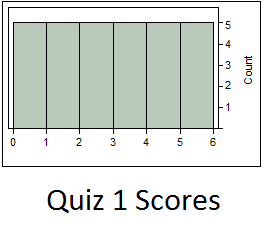
\includegraphics[keepaspectratio=TRUE,width=.2\textwidth]{figure/QuizScores1Version1.png}
% 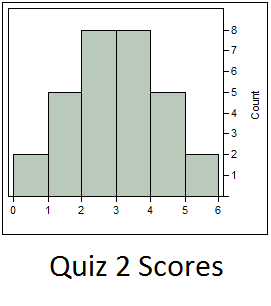
\includegraphics[keepaspectratio=TRUE,width=.2\textwidth]{figure/QuizScores2Version1.png}
% \end{center}
% \end{figure}
% %-------------------------------------------------------
% %\section{Appendix on Bivariate MANCOVA Model Specifications}
% %\label{ModelSpec}
% %-------------------------------------------------------
% %-------------------------------------------------------
% \section{Appendix of MANCOVA Model Diagnostics}
% \label{appModDiag}
% 
% For the ARTIST Model described in Subsection~\ref{ArtistModel} and the Applied Model described in Subsection~\ref{AppliedModel} a set of model diagnostics were conducted. Each of these MANCOVA models are parameterized as specified in Section~\ref{analysis}; as such the assessment of model assumptions will be very similar for each model. First, repercussions of violating the assumption of independence are assessed through a simulation study.  Residual plots will be used to assess the assumptions of linearity and constant variance.  The univariate and bivariate normality of the error terms will be assessed visually using normal quantile plots and a scatterplot of the paired residuals from the model. Additionally, although it is not a modeling assumption, MANCOVA models are best behaved with low to moderate correlation between the response variables, because then then model is able to capture variance unique to each response. 
% 
% \subsection{Appendix of Simulation Study for Violations of Independence}
% \label{simappend}
% 
% The assumption of independence of errors between students in the bivariate MANCOVA models specified in  (\ref{eq:mancova}), which we employed in Sections~\ref{ArtistModel}~and~\ref{AppliedModel} , is made in order to fit models with parsimonious variance structures. The assumption of independence between students is very likely violated in practice, because learning outcomes for students attending the same class with the same instructors in the same semester could well be related. It is therefore important to assess the consequences this violation has on the results of the MANCOVA models fit in the paper.  We wish to identify the effect of the violation on the error rates in the tests for curriculum effects on the learning outcomes. We elected to explore the consequences through a simulation study wherein the assumption of independence was knowingly violated and the effects on errors rates were recorded.
% 
% We chose the ARTIST Model (\ref{eq:mancova}) from Sections~\ref{ArtistModel} as the basis for our simulation study. Under the assumption of independence in the errors between students, we found weak evidence of a curriculum effect on the bivariate learning outcomes based on Pillai's $\lambda$. Further inspection of the individual responses using t-tests revealed evidence of a significant effect of the curriculum on confidence interval related outcomes, but no evidence of a curriculum effect on hypothesis test related outcomes.  In order to assess the reliability of the results, we must first know how a violation of the assumption of independence would impact the error rates for these tests.  We simulate under the scenario where the curriculum effect on learning outcomes is non-existent and assess the effect on   error rates under differing degrees of violation. 
% 
% The ARTIST Model of the form  (\ref{eq:mancova}) assumes  that errors from different students are independent, i.e.~$\Cov[\epsilon_{ik}, \epsilon_{jl}] = 0$, for all $i \neq j$ with $ 1 \le i,j \le n$. In our simulation setting, we simulate data from a model adapted from the model~(\ref{eq:mancova}), where there is no curriculum effect, i.e.~$\tau_{1} =  \tau_{2} = 0$ and where additionally the assumption of independent errors is violated by assuming a between student covariance of 
% \[
% \Cov[\epsilon_{ik}, \epsilon_{jl}] = \eta \sigma_{kl}^2, \ \ \ \text{ where } \eta \in [0,1]  \text{ for all } i \ne j. 
% \]
% $\eta$ scales the covariance between all students uniformly and can be adjusted to increase the violation of independence. Note that when $\eta = 0$ we have no violation of independence. Thus our generative model for the ARTIST responses are linear combinations of the midterm and lab~5 scores with correlated errors. This generative model for simulation can be organized using vector notation as follows:
% %
% \begin{eqnarray}\label{eq:linear}
% \begin{bmatrix}
%   \vec{y}_1 \\ \vec{y}_2
%   \end{bmatrix}  = 
% % %---- 
% \begin{bmatrix}
%  y_{11} \\ \vdots \\ y_{n1} \\ y_{12} \\ \vdots \\ y_{n2} 
% \end{bmatrix}  =
% % %----  
%  \begin{bmatrix}
%   \beta_{01} + x_{11}\beta_{11} + x_{12}\beta_{21}  \\
%   \vdots  \\ 
%   \beta_{01} + x_{n1}\beta_{11} + x_{n2}\beta_{21}  \\
%   \beta_{02} + x_{11}\beta_{12} + x_{12}\beta_{22}  \\
%   \vdots  \\ 
%   \beta_{02} + x_{n1}\beta_{12} + x_{n2}\beta_{22}  \\
%  \end{bmatrix} +
%  \begin{bmatrix}
%  \epsilon_{11} \\ \vdots \\ \epsilon_{n1} \\ \epsilon_{12} \\ \vdots \\ \epsilon_{n2} 
%  \end{bmatrix} = 
%  % %----
%  \begin{bmatrix}
%   X\vec{\beta}_1 \\ X\vec{\beta}_2
%   \end{bmatrix} + 
%   \vec{\epsilon},
% \end{eqnarray} 
% %
% \begin{eqnarray}\label{eq:error}
% \vec{\epsilon} \sim
% % %----  
%  \text{MVN}\left(
% \vec{0} \hspace{.1cm}
%   , 
%   \begin{bmatrix}
%    \sigma_{11}^2 & \sigma_{12}^2 \\ 
%    \sigma_{21}^2 & \sigma_{22}^2
%   \end{bmatrix}
% \otimes
%  \left( \eta 1_{n \times n} + (1- \eta) I_{n \times n}\right)
% %  \left[\begin{array}{ccccc|ccccc}
% %   \sigma_{11}^2 & \eta \sigma_{11}^2 & \cdots & \eta \sigma_{11}^2 & \eta \sigma_{11}^2 & \sigma_{12}^2 & \eta \sigma_{12}^2 & \cdots & \eta \sigma_{12}^2 & \eta \sigma_{12}^2\\
% %   \eta \sigma_{11}^2 & \sigma_{11}^2 & \ddots & \eta \sigma_{11}^2 & \eta \sigma_{11}^2 & \eta \sigma_{12}^2 & \sigma_{12}^2 & \ddots & \eta \sigma_{12}^2 & \eta \sigma_{12}^2\\
% % \vdots & \ddots & \ddots &\ddots &\vdots & \vdots & \ddots & \ddots &\ddots &\vdots \\
% % \eta \sigma_{11}^2 & \eta \sigma_{11}^2 & \ddots & \sigma_{11}^2 & \eta \sigma_{11}^2 & \eta \sigma_{12}^2 & \eta \sigma_{12}^2 & \ddots & \sigma_{12}^2 & \eta \sigma_{12}^2\\
% % \eta \sigma_{11}^2 & \eta \sigma_{11}^2 & \cdots & \eta \sigma_{11}^2 & \sigma_{11}^2 & \eta \sigma_{12}^2 & \eta \sigma_{12}^2 & \cdots & \eta \sigma_{12}^2 & \sigma_{12}^2\\
% % \hline
% % \sigma_{12}^2 & \eta \sigma_{12}^2 & \cdots & \eta \sigma_{12}^2 & \eta \sigma_{12}^2 & \sigma_{22}^2 & \eta \sigma_{22}^2 & \cdots & \eta \sigma_{22}^2 & \eta \sigma_{22}^2\\
% %   \eta \sigma_{12}^2 & \sigma_{12}^2 & \ddots & \eta \sigma_{12}^2 & \eta \sigma_{12}^2 & \eta \sigma_{22}^2 & \sigma_{22}^2 & \ddots & \eta \sigma_{22}^2 & \eta \sigma_{22}^2\\
% % \vdots & \ddots & \ddots &\ddots &\vdots & \vdots & \ddots & \ddots &\ddots &\vdots \\
% % \eta \sigma_{12}^2 & \eta \sigma_{12}^2 & \ddots & \sigma_{12}^2 & \eta \sigma_{12}^2 & \eta \sigma_{22}^2 & \eta \sigma_{22}^2 & \ddots & \sigma_{22}^2 & \eta \sigma_{22}^2\\
% % \eta \sigma_{12}^2 & \eta \sigma_{12}^2 & \cdots & \eta \sigma_{12}^2 & \sigma_{12}^2 & \eta \sigma_{22}^2 & \eta \sigma_{22}^2 & \cdots & \eta \sigma_{22}^2 & \sigma_{22}^2\\  
% %  \end{array}\right]
%  \right),
% \end{eqnarray}
% where $A \otimes B = \left( a_{ij} B \right)$ is the Kronecker product of matrices $A$ and $B$. $\vec{0}$ is the zero vector of length $2n$, $1_{n\times n}$ is the $n \times n$ matrix consisting of 1s only, and $I_{n \times n}$ is the identity matrix of dimension $n \times n$.
% Here, $x_{i1}$ is the midterm exam score for student $i$ and $x_{i2}$ is the lab~5 score for student $i$. In order to achieve practically relevant values for the coefficients $\beta_{kp}$ of the generative model we selected the estimated values from a MANCOVA model fit to the ARTIST responses using only the midterm exam and lab~5 scores.  Likewise, the variance components, $\sigma_{kl}$ for the generative model were selected using the estimated variance structure from the same reduced MANCOVA model for the ARTIST responses. 
% 
% The simulation procedure for assessing the error rates under violation independence between student responses was conducted in a five step process.
% For each $\eta$ in $\{0,0.1,0.2,0.3,0.4,0.5\}$ repeat the following process for $M = 25,000$ simulations each:
% %
% \begin{enumerate}
% \item Simulate an error vector, $\vec{\epsilon}^{\hspace{.1cm}(m)}$, from the multivariate normal distribution as defined in~(\ref{eq:error}).
% \item Derive corresponding responses based on model (\ref{eq:linear}) as:
% %
% \[
% \begin{bmatrix}
%   \vec{y}_1^{\hspace{.1cm}(m)} \\ \vec{y}_2^{\hspace{.1cm}(m)}
%   \end{bmatrix}   =
%    % %----
%  \begin{bmatrix}
%   X\vec{\beta}_1 \\ X\vec{\beta}_2
%   \end{bmatrix} + 
%   \vec{\epsilon}^{\hspace{.1cm}(m)}
% \]
% %
% \item Create assignment to curricula  for each student randomly. 
% 
% \item Fit the ARTIST Model (assuming independence) as given in model (\ref{eq:mancova}) to the simulated responses
% \item Record $\hat{\beta}_{kp}^{\hspace{.1cm}(m)}$, $\text{SE}\left[\hat{\beta}_{kp}^{\hspace{.1cm}(m)}\right]$, $\tau_k^{\hspace{.1cm}(m)}$, $\text{SE}\left[\tau_k^{\hspace{.1cm}(m)}\right]$ and $\hat{\sigma}_{kl}^{\hspace{.1cm}(m)}$ $\forall k,l \in \{1,2\}$ and $p \in \{0,1,2\}$. \\
% Also record Pillai's $\lambda^{\hspace{.1cm}(m)}$ testing for overall curriculum effect.
% %\item Repeat simulation steps 1 through 6, $M=25000$ times
% 
% \end{enumerate}
% 
% <<results, echo=FALSE, include=FALSE>>=
% load("C:\\Users\\Karsten\\Dropbox\\Dissertation\\CurriculumStudy\\SimulationStudy\\SimulationResults.RData")
% library(plyr)
% eta <- (0:5)/10
% results <- ldply(1:6, function(x) data.frame(eta=eta[x], resultlist[[x]]))
% # beta1s and beta2s are actually tau1 and tau2
% simresults = ddply(results, .(eta), summarise,
%       trt1=mean(beta1s),
%       trt2=mean(beta2s),
%       type1.1=mean(pval1s<0.05),
%       type1.2=mean(pval2s<0.05),      
%       betamidterm1s = mean(betamidterm1s),
%       pvalmidterms1s = mean(pvalmidterm1s),
%       sebetamidterm1s = mean(SEbetamidterm1s),
%       betamidterm2s = mean(betamidterm2s),
%       pvalmidterms2s = mean(pvalmidterm2s),
%       sebetamidterm2s = mean(SEbetamidterm2s),
%       avgpillai = mean(pillais),
%       avgpillaipval = mean(pillaipvals),
%       sebeta1s = mean(SEbeta1s),
%       sebeta2s = mean(SEbeta1s),
%       sdbeta1 = sd(beta1s),
%       sdbeta2 = sd(beta2s)
% )
% 
% 
% L <- length(resultlist)
% M = nrow(resultlist[[1]]) 
% errorsummary <- data.frame(T2ErrorRateBetaMidterm1 = rep(NA, L),
%                            T2ErrorRateBetaMidterm2 = rep(NA, L),
%                            T2ErrorRateBetaLab1 = rep(NA, L),
%                            T2ErrorRateBetaLab2 = rep(NA, L),
%                            T1ErrorRateBeta1 = rep(NA, L),
%                            T1ErrorRateBeta2 = rep(NA, L),
%                            T1ErrorRatePillai = rep(NA, L))
% 
% for (l in 1:L){
%   errorsummary[l,1] <- 1- length(which(resultlist[[l]]$pvalmidterm1s <= 0.05)) / M
%   errorsummary[l,2] <- 1- length(which(resultlist[[l]]$pvalmidterm2s <= 0.05)) / M
%   errorsummary[l,3] <- 1- length(which(resultlist[[l]]$pvallab1s <= 0.05)) / M
%   errorsummary[l,4] <- 1- length(which(resultlist[[l]]$pvallab2s <= 0.05)) / M
%   errorsummary[l,5] <- length(which(resultlist[[l]]$pval1s <= 0.05)) / M
%   errorsummary[l,6] <- length(which(resultlist[[l]]$pval2s <= 0.05)) / M
%   errorsummary[l,7] <- length(which(resultlist[[l]]$pillaipvals <= 0.05)) / M
% }
% errorsummary$eta <- eta
% #errorsummary
% @
% 
% Histograms for the estimated parameters from simulations at each value of $\eta$ are displayed in Figure~\ref{fig:simhistogrid}.  Note that the histograms are each centered around the true values of the parameters from the generative model, indicating that the estimates remain unbiased as the violation of independence between student responses increases. The figure also displays a decreasing variability in the parameter estimates as $\eta$ increases. The standard deviation for the treatment effect estimates, $s_{\tau_k}$, can be found in table~\ref{tab:simvarcompare}; along with averages from standard errors for the treatment effects, $\hat{\text{SE}}\left[\tau_k\right]$.  Note that while the former is measuring the variability of the coefficients from all simulations, the latter is the average of variability estimates from each individual simulation.  The paired values are nearly equivalent, meaning that the standard errors used in the t-tests for treatment effects shrink at the same rate as the true sampling variability in the parameters estimates as the violation of independence increases. 
% 
% <<simhistogrid, echo=FALSE , message=FALSE, warning=FALSE, fig.width=10, fig.height=6, out.width='1\\linewidth', fig.pos='h',fig.align='center',fig.cap="ARTIST model parameter estimates from 25,000 simulations at each $\\eta$. True parameter values from the generative model are displayed as vertical lines in each cell.", cache=TRUE>>=
% library(ggplot2)
% library(reshape2)
% etas <- seq(from=0, to=0.5, by=.1) 
% plotbetadata <- data.frame(eta = rep(as.character(etas),each=M))
% plotbetadata <- cbind(plotbetadata, rbind(resultlist[[1]][,c(1,2,7,8,13,14)],
%                                           resultlist[[2]][,c(1,2,7,8,13,14)],
%                                           resultlist[[3]][,c(1,2,7,8,13,14)],
%                                           resultlist[[4]][,c(1,2,7,8,13,14)],
%                                           resultlist[[5]][,c(1,2,7,8,13,14)],
%                                           resultlist[[6]][,c(1,2,7,8,13,14)]) )
% names(plotbetadata) <- c("eta","beta[11]","beta[12]","beta[21]","beta[22]","tau[1]","tau[2]")
% plotbetadata$eta <- paste("eta==",plotbetadata$eta,sep="")
% meltplotbetadata <- melt(plotbetadata, id=c("eta"))
% trueeffects <- unique(meltplotbetadata[,1:2])
% trueeffects$value <-  rep(c(0.046132,0.037915,0.017485, 0.008211,0,0),each=6)
% number_ticks <- function(n) {function(limits) pretty(limits, n)}
% qplot(value, geom="histogram", data=meltplotbetadata,fill=I("gray42")) + 
%   facet_grid(eta~variable, scales = "free",labeller = label_parsed) +
%   geom_vline(aes(xintercept = value), data=trueeffects, color="black")+ theme_bw()+
%   ylab("") + xlab("Estimated Parameter Values") +
%   scale_x_continuous(breaks=number_ticks(3))
% @
% 
% \begin{table}[hbtp]
% \centering
% \begin{tabular}{ccccc} \hline
% $\eta$ & $s_{\tau_1}$ & $\hat{\text{SE}}\left[\tau_1\right]$ & $s_{\tau_2}$ & $\hat{\text{SE}}\left[\tau_2\right]$\\ 
%  \hline  
% sprintf("%.1f",round(simresults[1,1],1)) & sprintf("%.4f",round(simresults[1,14],4)) & sprintf("%.4f",round(simresults[1,16],4)) &sprintf("%.4f",round(simresults[1,15],4))  &sprintf("%.4f",round(simresults[1,17],4)) \\
% sprintf("%.1f",round(simresults[2,1],1)) & sprintf("%.4f",round(simresults[2,14],4)) & sprintf("%.4f",round(simresults[2,16],4)) &sprintf("%.4f",round(simresults[2,15],4))  &sprintf("%.4f",round(simresults[2,17],4)) \\
% sprintf("%.1f",round(simresults[3,1],1)) & sprintf("%.4f",round(simresults[3,14],4)) & sprintf("%.4f",round(simresults[3,16],4)) &sprintf("%.4f",round(simresults[3,15],4))  &sprintf("%.4f",round(simresults[3,17],4)) \\
% sprintf("%.1f",round(simresults[4,1],1)) & sprintf("%.4f",round(simresults[4,14],4)) & sprintf("%.4f",round(simresults[4,16],4)) &sprintf("%.4f",round(simresults[4,15],4))  &sprintf("%.4f",round(simresults[4,17],4)) \\
% sprintf("%.1f",round(simresults[5,1],1)) & sprintf("%.4f",round(simresults[5,14],4)) & sprintf("%.4f",round(simresults[5,16],4)) &sprintf("%.4f",round(simresults[5,15],4))  &sprintf("%.4f",round(simresults[5,17],4)) \\
% sprintf("%.1f",round(simresults[6,1],1)) & sprintf("%.4f",round(simresults[6,14],4)) & sprintf("%.4f",round(simresults[6,16],4)) &sprintf("%.4f",round(simresults[6,15],4))  &sprintf("%.4f",round(simresults[6,17],4)) \\
% \hline
% \end{tabular}
% \caption{Comparison of the standard deviation for the treatment effect estimates, $s_{\tau_k}$, and average from standard errors for the treatment effects, $\hat{\text{SE}}\left[\tau_k\right]$ from simulations under each $\eta$.}
% \label{tab:simvarcompare}
% \end{table}
% %
% Table~\ref{tab:errorrates} displays that the Type I error rates from the Pillai's test and each of the individual t-tests for curriculum treatment effects are stable around the nominal $\alpha = 0.05$ level for all $\eta$ values. Thus the violation of independence between student responses is not detrimental to the Type I error rates in this setting, where no treatment effects exists in our generative model.  The stability in the Type I errors is linked to the finding that the variability estimates used in testing are shrinking at approximately the same rate as the true sampling variability in the parameters estimates, as discussed above.
% 
% Figure~\ref{fig:visual1} displays that the treatment effect estimates remain unbiased and the Type I error rates for testing the significance of the treatment on each response remain at the nominal level. We may additionally be curious about the Type II error rates; failing to find effects significant that truly exist in our generative model.  Figure~\ref{fig:visual2} displays that the midterm effect estimates are unbiased for the non-zero parameters in our generative model.  It also shows that the Type II error rate in fact \textit{decreases} as the dependence between student responses increases.  This implies that power for finding a truly significant effect \textit{increased} as the violation of independence increased.  
% 
% Our simulations, under this generative model, have demonstrated that parameter estimates remain unbiased and error rates are not detrimentally effected by increasing dependence between student responses.  Thus concerns over violating the modeling assumption of independence between student responses are alleviated. 
% 
% \begin{table}[hbtp]
% \centering
% \begin{tabular}{cccc} \hline
% $\eta$  & Pillai's Test & t-test (CI) & t-test (HT) \\
% & $\text{H}_o : \tau_1 = \tau_2 = 0$  & $\text{H}_o : \tau_1 = 0$ &  $\text{H}_o : \tau_2 = 0$\\ 
%  \hline  
% sprintf("%.1f",round(errorsummary[1,8],1)) & sprintf("%.4f",round(errorsummary[1,7],4)) & sprintf("%.4f",round(errorsummary[1,5],4)) &sprintf("%.4f",round(errorsummary[1,6],4)) \\
% sprintf("%.1f",round(errorsummary[2,8],1)) & sprintf("%.4f",round(errorsummary[2,7],4)) & sprintf("%.4f",round(errorsummary[2,5],4)) &sprintf("%.4f",round(errorsummary[2,6],4)) \\
% sprintf("%.1f",round(errorsummary[3,8],1)) & sprintf("%.4f",round(errorsummary[3,7],4)) & sprintf("%.4f",round(errorsummary[3,5],4)) &sprintf("%.4f",round(errorsummary[3,6],4)) \\
% sprintf("%.1f",round(errorsummary[4,8],1)) & sprintf("%.4f",round(errorsummary[4,7],4)) & sprintf("%.4f",round(errorsummary[4,5],4)) &sprintf("%.4f",round(errorsummary[4,6],4)) \\
% sprintf("%.1f",round(errorsummary[5,8],1)) & sprintf("%.4f",round(errorsummary[5,7],4)) & sprintf("%.4f",round(errorsummary[5,5],4)) &sprintf("%.4f",round(errorsummary[5,6],4)) \\
% sprintf("%.1f",round(errorsummary[6,8],1)) & sprintf("%.4f",round(errorsummary[6,7],4)) & sprintf("%.4f",round(errorsummary[6,5],4)) &sprintf("%.4f",round(errorsummary[6,6],4)) \\
% \hline
% \end{tabular}
% \caption{Type I error rates for tests for curriculum treatment effect from 25,000 simulations at each $\eta$. All tests were conducted with a nominal significance level of $\alpha = 0.05$.}
% \label{tab:errorrates}
% \end{table}
% 
% 
% <<visual1, echo=FALSE , message=FALSE, warning=FALSE, fig.width=11, fig.height=3, out.width='.9\\linewidth', fig.pos='h',fig.align='center',fig.cap="Average curriculum treatment effects on each value in the simulated response pairs (left) and corresponding Type I error rates (right) from 25,000 simulations at each $\\eta$. The generative model set $\\tau_1 = \\tau_2 = 0$ and tests for significance were run using $\\alpha = 0.05$">>=
% library(ggplot2)
% library(reshape2)
% library(gridExtra)
% srm <- melt(simresults, id.var="eta", measure.var=c("trt1", "trt2"))
% levels(srm$variable) <- c("ConfMC","HypMC")
% p1 <- ggplot(aes(x=eta, y=value, group=variable), data=srm) + 
%   geom_hline(yintercept=0.00, colour="grey50") + theme_bw() + 
%   geom_point(size=4, aes(shape=variable)) + geom_line(aes(ltype=variable)) + ylim(c(-0.01,0.01)) + 
%   ylab("Estimated Treatment Effect") + xlab(expression(eta)) +
%   theme(legend.position="none")
% 
% srm <- melt(errorsummary, id.var="eta", measure.var=c("T1ErrorRateBeta1", "T1ErrorRateBeta2"))
% levels(srm$variable) <- c("ConfMC","HypMC")
% p2 <- ggplot(aes(x=eta, y=value, group=variable), data=srm) + 
%   geom_hline(yintercept=0.05, colour="grey50") + theme_bw() + 
%   geom_point(size=4, aes(shape=variable)) + geom_line(aes(ltype=variable)) + ylim(c(0,0.06)) + 
%   ylab("Type I Error Rate") + xlab(expression(eta)) +
%   scale_shape_discrete(name="Treatment Effect", labels=c(expression(paste("  ",tau[1])),expression(tau[2]))) +
%   theme(legend.text = element_text(size = 12))
% 
% grid.arrange(p1,p2,nrow=1, widths=c(1,1.4))
% @
% 
% <<visual2, echo=FALSE , message=FALSE, warning=FALSE, fig.width=11, fig.height=3, out.width='.9\\linewidth', fig.pos='h',fig.align='center',fig.cap="Average midterm exam effects on each value in the simulated response pairs (left) and corresponding Type II error rates (right) from 25,000 simulations at each $\\eta$. The generative model set $\\beta_{11} = 0.0461$ and $\\beta_{12} = 0.0379 $ and tests for significance were run using $\\alpha = 0.05$.">>=
% srm <- melt(simresults, id.var="eta", measure.var=c("betamidterm1s", "betamidterm2s"))
% levels(srm$variable) <- c("ConfMC","HypMC")
% p1 <- ggplot(aes(x=eta, y=value, group=variable), data=srm) +
%   #geom_hline(yintercept=c(0.046132,0.037915), colour="grey50")+
%   theme_bw() + 
%   geom_point(size=4, aes(shape=variable)) + geom_line(aes(ltype=variable)) +
%   ylab("Estimated Midterm Effect") + xlab(expression(eta)) + ylim(c(0, 0.05))+
%   theme(legend.position="none")
% 
% 
% srm <- melt(errorsummary, id.var="eta", measure.var=c("T2ErrorRateBetaMidterm1", "T2ErrorRateBetaMidterm2"))
% levels(srm$variable) <- c("ConfMC","HypMC")
% p2 <- ggplot(aes(x=eta, y=value, group=variable), data=srm) + 
%   theme_bw() + 
%   geom_point(size=4, aes(shape=variable)) + geom_line(aes(ltype=variable)) +
%   ylab("Type II Error Rate") + xlab(expression(eta)) +
%   scale_shape_discrete(name="Midterm Coefficients", labels=c(expression(paste("  ",beta[11])),expression(beta[12]))) +
%   theme(legend.text = element_text(size = 12))
% grid.arrange(p1,p2,nrow=1, widths=c(1,1.4))
% @
% 
% 
% A final consideration is that in practice we might be dealing with a situation where there is a more complex covariance structure, where students of the same classrooms have more related scores than students of different classrooms. The rational is that students within the same physical environment may interact in ways that cause their responses to be more similar than students of different classrooms. In this situation we adjust the generative model (\ref{eq:linear}) to assume the covariance between student to be
% \[
% \Cov[\epsilon_{ik}, \epsilon_{jl}] = c \eta \sigma_{kl}^2, 
% \]
% where $c = 1$ for all students $i,j$ in same classroom, and $c \in [0,1] $ for students $i,j$ in different classrooms.  In this way, $c$ scales the covariance back for all students not sharing a classroom. We will refer to $c$ as the ``non-classmate covariance scaling parameter".  
% %We will bear in mind that this difference should not reflect a treatment effect, merely a covariance structure for items on the final exam due to the sharing of physical environments (i.e. inter-student conversation, physical differences in classroom).  We do not want $c$ to represent the differences caused by the administration of a curricula because this is considered a treatment effect, which is not supposed to exist in the generative model. We will simulate with $c$ rather close to 1 in the generative model.
% The simulation procedure otherwise follows the same five stage procedure described previously with $M = 10,000$ simulations at each combination of $\eta$ in $\{0,0.1,0.2,0.3,0.4\}$ and $c$ in $\{0.9, 0.925, 0.95, 0.975, 1.0\}$.
% 
% Similar to the initial simulation, it was found that the parameter estimates remain unbiased as the violation of independence between student responses increases in this adapted generative model. There was also decreasing variability in the parameter estimates as $\eta$ and $c$ increase.
% 
% Figure~\ref{fig:sim2plots} displays the Type I error rates for testing for treatment effects univariately using t-tests and bivariately using Pillai's overall test. What is clear is that the type I error rate climbs quickly when the non-classmate covariance scaling parameter decreases. This means that when the variance structure for observations more clearly aligns for students in the same classroom, it becomes more likely to observe a difference in the scores between classrooms.  
% 
% Unfortunately, there is no way to estimate $c$ from our data, where classroom is entirely confounded with curricula treatment.  As such we will need to recognize that reliability of our results are contingent on the belief that the alternation of instruction, identical curricula administered with all students in the same room in weeks 1 to 8, and careful pedagogical preparation has minimized all non-treatment related differences that may have arisen due to the physically different classrooms in which the treatments were administered.
% 
% <<ResultsClassroomSimulation, echo=FALSE, include=FALSE>>=
% errorsummary2 <- read.csv("C:\\Users\\Karsten\\Dropbox\\Dissertation\\CurriculumStudy\\SimulationStudy/Sim1000ClassCovResults.csv")
% @
% 
% <<sim2plots, echo=FALSE , message=FALSE, warning=FALSE, fig.width=8, fig.height=3, out.width='.8\\linewidth', fig.pos='h',fig.align='center',fig.cap="Type I error rates for tests of treatment effects from 10,000 simulations at each combination of $\\eta \\in \\{0,0.1,0.2,0.3,0.4\\}$ and $c \\in \\{0.9,0.925,0.95,0.975,1.0\\}$. The nominal $\\alpha=0.05$ is displayed with the dashed line in each plot.", cache=TRUE>>=
% library(ggplot2)
% meltsim2 <- melt(errorsummary2, id=c("eta", "nonclassmate"))
% meltsim2$variable2 <- factor(meltsim2$variable, labels = c("H[o]: tau[1]==0", "H[o]: tau[2]==0", "Pillai"))
% qplot(eta, value, geom="path", data=meltsim2, colour=as.factor(nonclassmate), group=nonclassmate, size=I(1.2)) +
%   geom_point(size=I(1.6),colour=("Black"))+
%    facet_grid(. ~ variable2, labeller = label_parsed) +
%   xlab(expression(eta)) + ylab("Type I Error Rate") + 
%   theme_bw() + labs(colour='Non-classmate Variance
% Scaling Parameter (c)') + geom_hline(yintercept=0.05, linetype=2)+
%    geom_hline(yintercept=0, linetype=1)+
%   ylim(c(0,.50))+
%   scale_colour_manual(values = c("gray80","gray70","gray60","gray60","gray40"))
% @
% 
% 
% 
% \subsection{ARTIST Model Diagnostics}
% \label{appARTISTModDiag}
% 
% 
% The ARTIST Model is assessed to satisfactorily meet the modeling assumptions. The correlation between the ARTIST scores for confidence intervals and hypothesis tests is acceptable for modeling with MANCOVA with a correlation of $round(with(dat, cor(ConfMC,HypMC)),3)$ between the responses.  The normality of the errors is upheld by the plots in Figure~\ref{fig:ARTISTModDiag}.  The normal quantile plots only display a slight bend for the residuals from the Hypothesis Test topic scores, and the bivariate distribution of the residuals are visually consistent with bivariate normality. 
% 
% <<ARTISTModDiag, echo=FALSE , warning=FALSE, fig.width=5, fig.height=5, out.width='.49\\linewidth', fig.pos='h',fig.align='center',fig.cap="Normal quantile plots (left) and bivariate scatterplot (right) for residuals of each response from ARTIST Model.",fig.show='hold'>>=
% #--------------------------------------------------
% ### Check Conditions for MANCOVA linear model fit
% ## check response correlations to avoid colinearity in multivariate model
% #Rule of Thumb: ~ .3 to .55 then MANCOVA will work well
% #with(dat, cor(ConfMC,HypMC)) #Not overly correlated
% 
% ### check for influencial and high leverage points
% #infmeas <- influence.measures(mod2small)
% #head(infmeas$infmat)
% #head(infmeas$is.inf)
% ### no high leverage
% 
% #Normality of Residuals
% #op <- par(mfrow = c(1, 3))      
% #qqp1 <- qqPlot(mod2small$residuals[,1], xlab="Theoretical Normal Quantiles",
% #       ylab="ARTIST CI Score Residual")
% 
% #qqp2 <- qqPlot(mod2small$residuals[,2], xlab="Theoretical Normal Quantiles",
% #       ylab="ARTIST HT Score Residual")
% #op
% 
% qqp1 <- qplot(sample=mod2small$residuals[,1], stat="qq", xlab="Theoretical Normal Quantiles",
%        ylab="ARTIST CI Score Residual") +  theme_bw()
% 
% qqp2 <- qplot(sample=mod2small$residuals[,2], stat="qq", xlab="Theoretical Normal Quantiles",
%       ylab="ARTIST HT Score Residual") +  theme_bw()
% 
% grid.arrange(qqp1,qqp2,nrow=2)
% 
% qplot(mod2small$residuals[,1],mod2small$residuals[,2],
%       xlab="ARTIST CI Score Residual",  ylab="ARTIST HT Score Residual")  +  theme_bw()
% # Univariate and Bivariate normality looks fine
% 
% # makeenv <- function(res){
% # grav.qqboot <- boot(res,sort,R=999,sim="parametric",ran.gen=grav.gen)
% # theo.qq <- qqnorm(res,plot=FALSE)
% # theo.qq <- lapply(theo.qq,sort)
% # env <- envelope(grav.qqboot,level=0.95)
% # envdat <- data.frame(theoquant = c(theo.qq$x,theo.qq$x),
% #                      envelope = c(env$point[1,],env$point[2,]),
% #                      bound = rep(c("upper","lower"),each=length(res)))
% # return(envdat)
% # }
% # 
% # envdat <- makeenv(mod2small$residuals[,1])
% # head(envdat)
% # qplot(sample = mod2small$residuals[,1], stat = "qq") +
% #   geom_path(aes(x=theoquant, y=envelope), data=subset(envdat,bound=="lower")) +
% #   geom_path(aes(x=theoquant, y=envelope), data=subset(envdat,bound=="upper"))
%   
%   
% ## Independence of responses between students must be assumed
% @
% 
% The residual plots in Figure~\ref{fig:residualsARTIST} display stripped bands of points that run shallowly downward, creating the optical illusion of a trend in the points.  This is because the model fits the discretely recorded ARTIST scores as continuous response variables, thus there is a discrete set of residuals possible for any particular fitted value.  Note that, as with all least-squares regression models, the residuals are uncorrelated with the fitted values. 
% 
% The residual plots in Figure~\ref{fig:residualsARTIST} are overlain with Loess smoothers -- and corresponding 95\% confidence envelopes -- to check for violations of linearity.  There is no issue with the assumption of linearity in the prediction of the confidence interval score, but there is a slight significant dip in the pattern for hypothesis interval residuals.  The assumption of homoscedasticity appear to hold with the residuals spread fairly evenly at all levels of the fitted values. There are however a few outliers on the residual plots, specifically a few students who scored abnormally lower than predicted. These outliers were investigated and found to be low leverage and non-influential. 
% 
% <<residualsARTIST, echo=FALSE , message=FALSE, warning=FALSE, fig.width=8, fig.height=3.2, out.width='.9\\linewidth', fig.pos='h',fig.align='center',fig.cap="ARTIST Model residual plots overlaid with Loess smoother and corresponding 95\\% confidence envelopes.">>=
% ## check residual plots for homoscedesticity and linearity
% jitheight <- .1
% p1 <- qplot(mod2small$fitted.values[,1] ,mod2small$residuals[,1], geom = "jitter") + 
%   geom_hline(yintercept=0) +geom_jitter(position = position_jitter(height = jitheight )) +
%   xlab("ARTIST CI Score Fitted Value") + ylab("ARTIST CI Score Residual") +  theme_bw() + geom_smooth()
% p2 <- qplot(mod2small$fitted.values[,2] ,mod2small$residuals[,2]) + 
%   geom_hline(yintercept=0) +geom_jitter(position = position_jitter(height = jitheight )) +
%   xlab("ARTIST HT Score Fitted Value") + ylab("ARTIST HT Score Residual") +  theme_bw() + geom_smooth()
% grid.arrange(p1,p2,nrow=1)
% # these seem fine (put into appendix)
% @
% 
% \subsection{Applied Model Diagnostics}
% \label{appAppliedModDiag}
% 
% A correlation of $round(with(dat, cor(AppliedCI,AppliedHT)),3)$ between the pair of applied problem scores for confidence intervals and hypothesis tests is acceptable for modeling with MANCOVA.  The assumption of normality of errors in the Applied Model is potentially problematic. The normal quantile plot for the residuals from the applied confidence interval score in Figure~\ref{fig:AppliedModDiag} show a distinct curve. The scatterplot of the residual pairs from the Applied Model also appear to have a non-normal bivariate distribution.
% 
% The Loess smoothers do not significantly departing from a the horizontal lines at zero for the residual plots in Figure~\ref{fig:residuals2} and thus no departures from the assumption of linearity.  The residuals do however show signs of changing variance over the range of the fitted values. This appears to be driven by the upper bound on student scores for each question.
% 
% <<AppliedModDiag, echo=FALSE , warning=FALSE, fig.width=5, fig.height=5, out.width='.49\\linewidth', fig.pos='h',fig.align='center',fig.cap="Normal quantile plots (left) and bivariate scatterplot (right) for residuals of each response from Applied Model.",fig.show='hold'>>=
% #--------------------------------------------------
% ### Check Conditions for MANCOVA linear model fit
% ## check response correlations to avoid colinearity in multivariate model
% #Rule of Thumb: ~ .3 to .55 then MANCOVA will work well
% #with(dat, cor(AppliedCI,AppliedHT)) #Not overly correlated
% 
% ### check for influencial and high leverage points
% #infmeas <- influence.measures(mod1small)
% #head(infmeas$infmat)
% #head(infmeas$is.inf)
% ### no high leverage
% 
% qqp1 <- qplot(sample=mod1small$residuals[,1], stat="qq", xlab="Theoretical Normal Quantiles",
%        ylab="Applied CI Score Residual") +  theme_bw()
% 
% qqp2 <- qplot(sample=mod1small$residuals[,2], stat="qq", xlab="Theoretical Normal Quantiles",
%       ylab="Applied HT Score Residual") +  theme_bw()
% 
% grid.arrange(qqp1,qqp2,nrow=2)
% 
% qplot(mod1small$residuals[,1],mod1small$residuals[,2],
%       xlab="Applied CI Score Residual",  ylab="Applied HT Score Residual")  +  theme_bw()
% @
% 
% 
% <<residuals2, echo=FALSE , warning=FALSE, message=FALSE, fig.width=8, fig.height=3.2, out.width='.9\\linewidth', fig.pos='H',fig.align='center',fig.cap="Applied Model residual plots overlaid with Loess smoother and corresponding 95\\% confidence envelopes.">>=
% p1 <- qplot(mod1small$fitted.values[,1] ,mod1small$residuals[,1]) + 
%   geom_hline(yintercept=0) +geom_jitter(position = position_jitter(height = jitheight )) +
%   xlab("Applied CI Score Fitted Value") + ylab("Applied CI Score Residual") +  theme_bw() + geom_smooth()
% p2 <- qplot(mod1small$fitted.values[,2] ,mod1small$residuals[,2]) + 
%   geom_hline(yintercept=0) +geom_jitter(position = position_jitter(height = jitheight )) +
%   xlab("Applied HT Score Fitted Value") + ylab("Applied HT Score Residual") +  theme_bw() + geom_smooth()
% grid.arrange(p1,p2,nrow=1)
% @
